\documentclass[11pt,a4paper]{book}
\usepackage[utf8]{inputenc}
\usepackage[T1]{fontenc}
\usepackage[spanish]{babel}
\usepackage{amsmath}
\usepackage{amsfonts}
\usepackage{amssymb}
\usepackage{graphicx}
\usepackage{fancyvrb}
\usepackage{float}
\usepackage{url}
\author{Ángel Perea Arias}
\newcommand{\mychapter}[2]{
	\setcounter{chapter}{#1}
	\setcounter{section}{0}
	\chapter*{#2}
	\addcontentsline{toc}{chapter}{#2}
}
\begin{document}
	\title{¡¡¡¡¡ Título temporal !!!!!}
	\date{24 de Mayo del 2020}
	\maketitle
	
	
	\tableofcontents
	%\listoftables
	\listoffigures
	\glossary{GLOSARIO?}
	
	\mychapter{0}{ÍNDICE DE CONTENIDOS}
	\mychapter{0}{ÍNDICE DE FIGURAS}
	\mychapter{0}{ÍNDICE DE TABLAS}
	\mychapter{0}{GLOSARIO}
	\chapter{INTRODUCCIÓN}
		\section{Resumen}
		\section{Motivación}
		El objetivo principal es dotar a la Web Kibotics.org de sondas de almacenamiento de datos y herramientas de visualización para el análisis de estos, ya sean de visitantes a la web, registros de usuarios o uso de los ejercicios.\\
		
		Ofreciendo así a la web y sus administradores de capacidades para recoger, estudiar y valorar los datos aportados para tener una mejor visión global de que rumbo tomar, como está funcionando el servicio, como mejorarlo. \\
		
		Estos datos son imprescindibles para cualquier decisión importante que se deba tomar para mejorar la satisfacción de los usuarios, aumentar la retención, mejorar los contenidos y su distribución etc... (INCOMPLETO)
	\chapter{OBJETIVOS}
	\chapter{INFRAESTRUCTURA UTILIZADA}
		En este capítulo se describen las diferentes tecnologías web, de bases de datos y de visualización que se han utilizado en el transcurso del proyecto.
		\section{Tecnologías Web}
			
			El desarrollo de sitios web o aplicaciones \textit{online} es un ámbito muy amplio con un gran abanico de tecnologías a disposición de los desarrolladores. En esta sección se explorarán las tecnologías web envueltas en el desarrollo del proyecto tanto en el lado cliente como servidor.
			\begin{figure}[H]
				\centering
				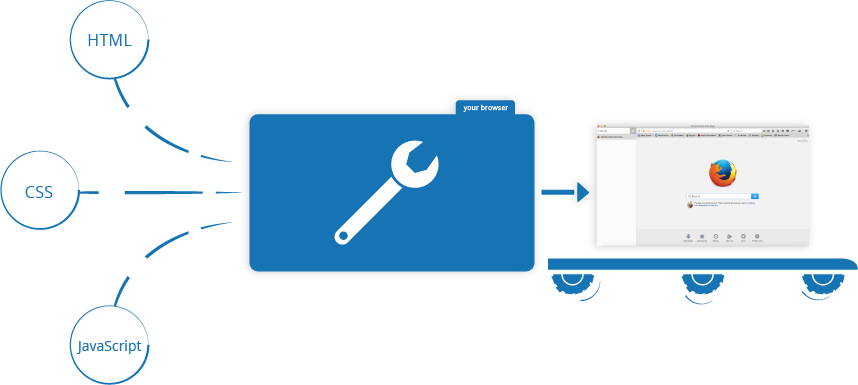
\includegraphics[width=10cm, keepaspectratio]{img/html_css_js.png}
				\caption{Tecnologías web básicas.}
				\label{fig:HTML_CSS_JS}
			\end{figure}
	
			\subsection{HTML}
				HTML (Hipertextual Markup Lenguaje) \cite{HTML}, es un lenguaje de marcado. Actualmente utilizado para la definición de  estructura básica de los contenidos de una página web como vídeos, gráficos, texto... \\
				
				Publicado en 1991, su historia se remonta a 1980, cuando Tim Berners-Lee propuso un nuevo sistema para compartir ficheros. Actualmente se ha impuesto como el lenguaje estándar para dar formato a documentos, definido por el \textit{World Wide Web Consortium} (W3C), el cual ha ido evolucionando versión a versión adoptando todas las nuevas exigencias que ofrecen las webs actuales, tanto en el campo de los recursos multimedia como en el de interactividad.\\
				
				HTML se desarrolla haciendo uso de una estructura de etiquetas o \textit{tags}, dentro de las cuales se pueden incluir cada uno de los elementos que conforman una página web. Dispone de cierta capacidad para aportar estilo y lógica pero estas generalmente se delegan en CSS y JavaScript respectivamente.\\
				
				La última versión oficial es HTML5, la cual proporciona soporte nativo para audio y vídeo, inclusión de la etiqueta \texttt{canvas} usada para generar gráficos y efectos tanto en 2D como en 3D, entre otras mejoras. Es la versión usada en este proyecto.
				
			\subsection{CSS}
				CSS (Cascade Style Sheet), es un lenguaje de reglas en cascada utilizado para dotar de diseño gráfico a elementos de una página web. Define, como se mencionó anteriormente, la estética de un documento HTML y por lo tanto de una página Web. \\
				
				Permite crear webs atractivas y responsivas, que se adapten al dispositivo en que están siendo vistas, ya sea por ejemplo, tabletas, ordenadores o móviles.\\
				
				Permite mover todas las reglas de estilo (tamaños de fuente o de imágenes, colores, responsividad de elementos a ciertas resoluciones...) a ficheros \texttt{*.css}, evitando así redundancia en un mismo documento \texttt{*.html}, mejorando así la modularidad e independencia dentro de un proyecto.\\
								
				La última versión es CSS3, añade novedades como soporte nativo para transiciones y animaciones. Además de herramientas para una maquetación más precisa. Es la versión usada en este proyecto.
				
			\subsection{JavaScript}
				JavaScript \cite{JavaScript} es un lenguaje de programación ligero, interpretado, orientado a objetos y dinámico. Utilizado principalmente como lenguaje de \textit{scripting} para paginas web, en este campo su papel principal se centra en el desarrollo de lógica en la parte del cliente \textit{backend}: acceso al \textit{Document Object Model}(DOM) de la web, modificación de etiquetas HTML, generación de gráficos en \textit{canvas} o gestión de \textit{cookies}.\\
				
				Permite crear nuevo contenido dinámico, así como controlar archivos multimedia y gracias al uso de API's (Aplication Programming Interface), enriquece a JavaScript con más funcionalidades permitiendo crear funcionalidades más complejas con desarrollos más simples.
				
			\subsection{Python}
				Python es un lenguaje de programación interpretado, orientado a objetos y de alto nivel. Diseñado para un desarrollo de aplicaciones rápido, se utiliza como lenguaje de \textit{scripting} y conexión entre otros componentes de un sistema.\\
				
				Python es simple, con una sintaxis fácil de aprender centrada en la legibilidad del código, consiguiendo así reducir el coste del desarrollo, mantenimiento y ampliación de proyectos.\\
				
				Tiene una gran biblioteca de librerías que puede ser fácilmente extendida por módulos personalizados escritos en C/Python. Haciendo uso del instalador de paquetes \texttt{PIP} (Python Package Installer), es posible la instalación e integración de paquetería en proyectos de manera muy sencilla, así como el cambio de versiones de las mismas.\\
				
				Pese a no ser estrictamenta hablando una tecnología web, en este proyecto lo hemos empleado en el contexto de Django, para programar la lógica \textit{backend}. El proyecto comenzó a desarrollarse en Python 2.6 y ha terminado en la versión Python 3.6.9.
				
				
			\subsection{Django}
				Django es un entorno Web de alto nivel diseñado para desarrollar servidores en Python. Al igual que este, su filosofía se centra en desarrollos rápidos, limpios y en un diseño pragmático. Sigue el patrón \textit{Model-View-Template} (MVT) \cite{Django MVC}, donde:\\
				
				\begin{itemize}
					\item \textit{Model}, esta capa del patrón tiene toda la información relativa a las bases de datos: cómo se almacenan, cómo se relacionan entre ellas, cómo validarlas... Manejado por la capa de bases de datos de Django. Toda esta información de configuración se desarrolla y almacena en el fichero \texttt{Models.py}. Mediante su ORM (Object Relational Model) permite al desarrollador del servidor hacer consultas y manejar los datos de bases de datos relacionales en Python. Los filtros, desarrollados en Python, se traducen automáticamente peticiones \texttt{SQL}.\\
					
					\item \textit{View}, parte lógica del Framework, se puede ver como una unión entre la capa de modelo y plantillas. Formado por dos ficheros: \texttt{urls.py}, encargado de llamar a la vista adecuada dependiendo de la URL a la que se acceda y \texttt{views.py} con todas esas vistas que devolverán una respuesta HTTP y en las cuales se consultará la capa Model si fuese necesario.\\
					
					
					\item \textit{Template}, sección que se encargará del qué y cómo mostrar los datos. Manejado por vistas y plantillas de Django que servirán de bases para la parte \textit{frontend} de la Web. Guardado en documentos HTML enriquecidos junto a variables de plantillas Django (\{\{ nombre\_de\_variable \}\}), las cuales permite el uso de, por ejemplo, bucles, operaciones condicionales, diccionarios, inserción de bloques... para generar webs enriquecidas y dinámicas en muy pocas líneas de código.
					
				\end{itemize}
			
				\begin{figure}[H]
				 	\centering
				 	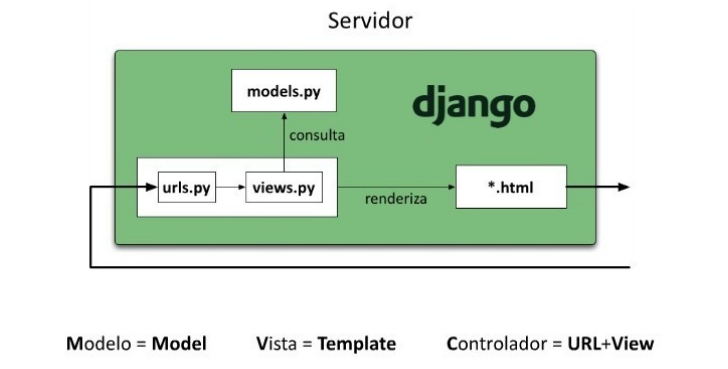
\includegraphics[width=13cm, keepaspectratio]{img/django_MTV.png}
				 	\caption{Patrón MVT Django.}
				 	\label{fig:MTV_Django}
				 \end{figure}
			 
			 	Diseñado para ser seguro, y evitar errores comunes, Django ofrece una fácil administración de las cuentas de usuarios, así como de sus contraseñas. Además de una sección de administración en la que poder gestionar toda la información almacenada en las bases de datos desplegadas.\\
			 	
			 	
				El software ya existente de Kibotics Webserver, servicio web sobre el que se ha trabajado, ya estaba basado en Django. El proyecto comenzó a desarrollarse en la versión 1.9 y ha concluido en la Django 1.11  \cite{Django}.
											
				
		\section{Bases de datos}
			Una base de datos es un conjunto de información, la cual pertenece a un mismo contexto, almacenada de modo sistemático y preservada en distintos formatos, puede ser consultada o alterada posteriormente. En esta sección, se detallarán las distintas tecnologías de bases de datos utilizadas en el desarrollo de este proyecto.
			\subsection{SQLite}
				SQLite es una librería ligera, rápida y fiable desarrollada en C. Siendo actualmente el motor de bases de datos SQL más usado en el mundo, utilizado en gran parte de los dispositivos móviles y ordenadores, además de venir de serie en muchas aplicaciones, por ejemplo, Django.\\
				
				
				No necesita de un servidor para funcionar, hecho por el cual su integración y despliegue es sencillo. Está basado en lectura y escritura en un fichero \texttt{*.sqlite} para almacenar toda la información de una base de datos. Este fichero es multiplataforma pudiendo así ser migrado entre distintos sistemas de manera muy sencilla, y tiene un tamaño máximo de 140 terabytes.\\
								
				\textbf{Versión? para qué nosotros? URL?}
				
			\subsection{MongoDB}
				MongoDB \cite{MongoDB} es una base de datos NoSQL (Not only SQL) distribuida, documental (almacenando la información en ficheros BSON, muy similares a JSON), de código abierto y diseñada para ofrecer un nivel productivo alto.\\
				
				Al ser una base de datos NoSQL, permite almacenar información de forma estructurada, pero flexible, pues los esquemas pueden ser cambiados sin necesidad de parar el servicio.
				
				Debido a esta estructura, la velocidad en las consultas es muy alta, convirtiéndose así en una base de datos ideal para trabajar con grandes cantidades de información que vayan a ser consultados muy frecuentemente.\\
				
				La escalabilidad de MongoDB es sencilla, puesto que se ejecuta en \textit{clusters}, podrá escalar horizontalmente contratando más máquinas, aumentando así la capacidad de procesamiento. Es una base de datos muy utilizada en la industria \cite{Use_MongoDB}.\\
							
				Para el primer prototipo de este proyecto, se ha utilizado la última versión estable de MongoDB, la versión 4.2.6.
				
			\subsection{Elasticsearch}
				Elasticsearch \cite{elasticseach} es una base de datos. Junto a Logstash y Kibana, los tres proyectos open source, forman el stack ELK. \\
				
				\begin{figure}[H]
					\centering
					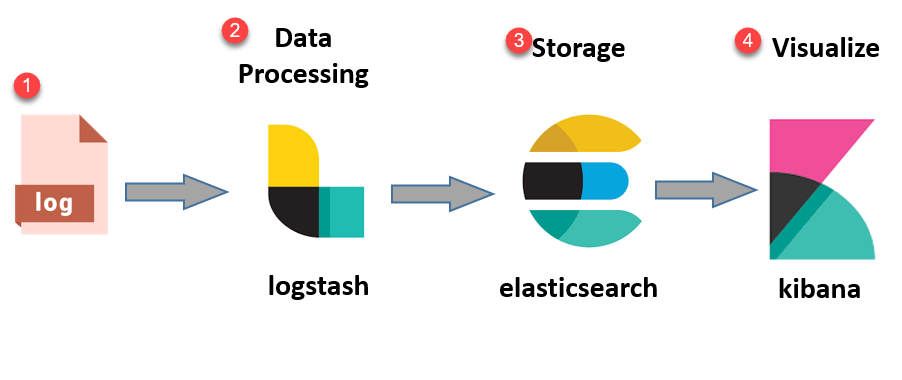
\includegraphics[width=10cm, keepaspectratio]{img/ELK_Stack.png}
					\caption{Stack ELK.}
					\label{fig:ELK_Stack}
				\end{figure}
			
				Basado en Lucene (API para recuperación de información), permite almacenar información compleja como datos de geolocalización así como realizar búsquedas de texto y auto-completado casi en tiempo real. Mediante el uso de una API Rest realiza consultas, borrado y actualización de documentos.\\
										
				En vez de usar filas y columnas, Elasticsearch almacena estructuras complejas de datos serializadas como documentos JSON. Para almacenar estos documentos, Elasticsearch hace uso de índices. Cada uno de estos índices dispone de una estructura de datos propia. Estas estructuras JSON son tambien utilizadas tanto para las consultas y respuestas, lo que la hace sencilla de usar e integrar en sistemas productivos ya existentes.\\
								
				Dadas estas capacidades de almacenar información preparada en índices, la consulta de documentos es muy ágil puesto que evita búsquedas tanto en indices como en documentos no deseados. Organizado en nodos, permitirá aumentar la potencia a medida que la demanda de recursos crezca. \\
				
				Se ha convertido en uno de los buscadores por texto más importantes, utilizado por gigantes de Internet como Facebook, Netflix o Github. \\
				
				La última versión estable de Elasticsearch es la versión 7.8.0 \cite{versions_elasticsearch}, liberada el 18 de Junio del 2020. En proyecto, se ha utilizando la versión 7.6.2 publicada el 31 de Marzo del 2020.


		
		\section{Tecnologías de visualización}
			La muestra de datos es una de las bases de este proyecto, en esta sección se explicarán las tecnologías utilizadas tanto en el primer prototipo como en la versión final del módulo de analíticas desarrollado para este proyecto.
			
			\subsection{Matplotlib}
				Matplotlib es una librería de Python que se encarga de la generación de visualizaciones tanto estáticas como animadas. \\
				
				Proporciona gran variedad de visualizaciones como mapas de calor, gráficas de barras, histogramas... recordando a Matlab. Ofrece cierta capacidad de estilo y puede ser utilizada junto a otras librerías para generar visualizaciones aún más complejas y enriquecidas como mapas geográficos en los que se representa datos mediante latitud y longitud. \\
				
				\begin{figure}[H]
					\centering
					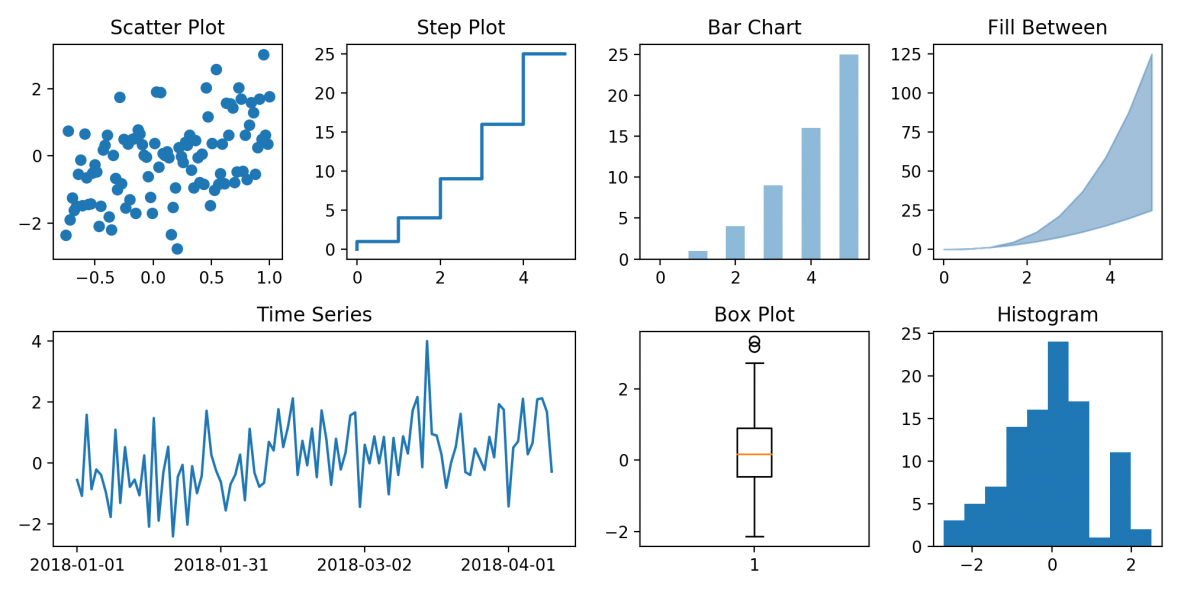
\includegraphics[width=11cm, keepaspectratio]{img/visualizations_matplotlib.png}
					\caption{Visualizaciones en Matplotlib.}
					\label{fig:visualizations_matplotlib}
				\end{figure}
			
				Matplotlib almacena las visualizaciones en figuras, cada una contiene los ejes en que se representarán los datos, estos ejes pueden ser de múltiples tipos, ya sean coordenadas x-y, x-y-x para una representación en tres dimensiones o un eje polar.\\
							
				Las visualizaciones generadas podrán ser mostradas en una nueva ventana si utilizamos la librería en un \textit{script} o ser renderizadas y devueltas como imagen \texttt{PNG} para su posterior muestra en el servicio web haciendo uso de la etiqueta \texttt{HTML} <img></img>\\
								
				En el primer prototipo de este proyecto se utilizó la versión 3.1.2 de Matplotlib, publicada el 18 de Marzo del 2020 \cite{releases_matplotlib}.
				
			\subsection{Kibana}
				Como se comentó anteriormente, el stack ELK está compuesto por Kibana \cite{kibana} como motor de búsqueda, procesador de datos y generador de visualizaciones entre otras funcionalidades. Diseñada para utilizar Elasticsearch como fuente de datos.\\
				
				Gracias a su aplicación \textit{frontend}, la creación de visualizaciones se simplifica mucho sin ser necesaria la codificación de estas. \\
				
				Mediante configuración, filtrado y selección de los datos indexados en Elasticsearch se pueden crear múltiples tipos de visualizaciones interactivas (gráficos de barras,  circulares, tablas, histogramas y mapas), y posteriormente ser agrupadas en tableros o \textit{Dashboards}, los cuales permiten la visualización y posterior filtrado de grandes cantidades de información de forma simultanea y sencilla.\\
								
				\begin{figure}[H]
					\centering
					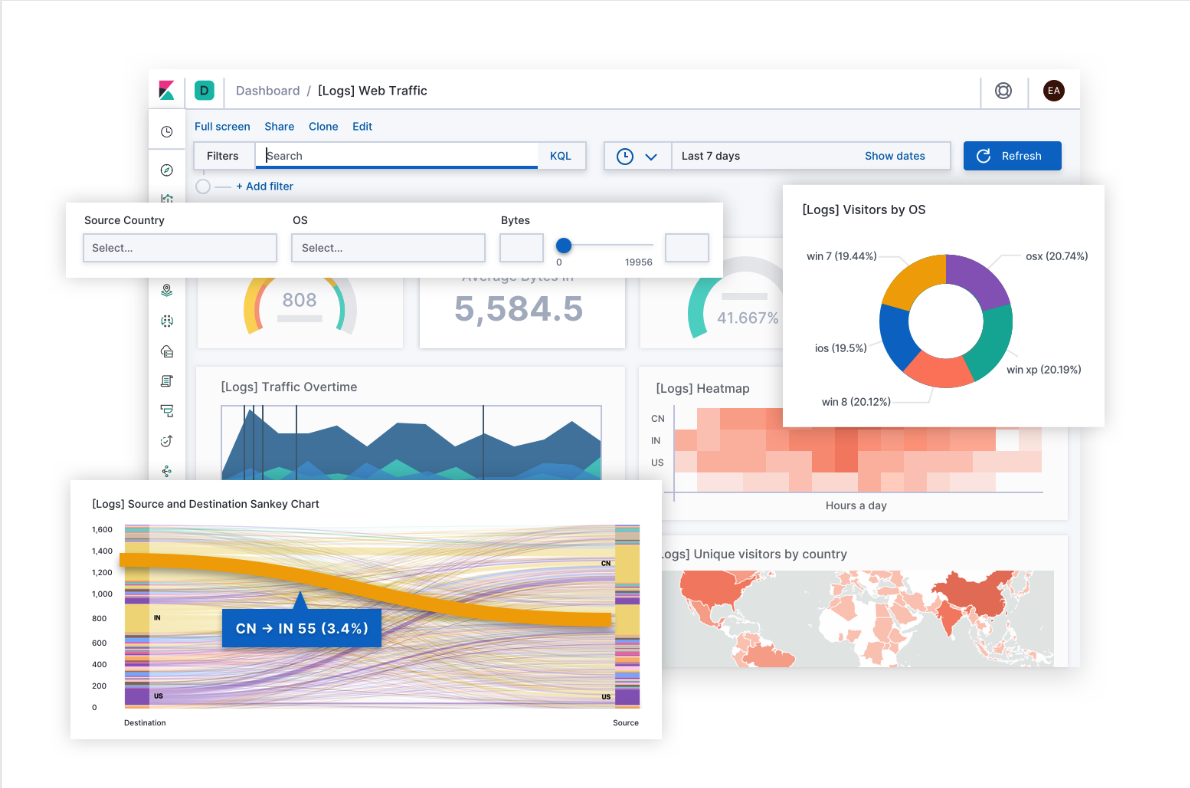
\includegraphics[width=12cm, keepaspectratio]{img/visualizations_kibana.png}
					\caption{Visualizaciones en Kibana.}
					\label{fig:visualizations_kibana}
				\end{figure}

				Permite el procesado de los documentos ya indexados en Elasticsearch para crear nuevos campos dinámicos que podrán ser utilizados y representados posteriormente en visualizaciones y estadísticas.\\
								
				Ofrece una interfaz segura y organizada, dividida en espacios de trabajo o \textit{spaces}. Estos espacios pueden ser tratados como instalaciones de Kibana independientes permitiendo a varios equipos de trabajo hacer uso del mismo servicio de Kibana sin los inconvenientes de compartir información de índices. Aumentando la compartimentalización y escalabilidad del servicio.
				
				\begin{figure}[H]
					\centering
					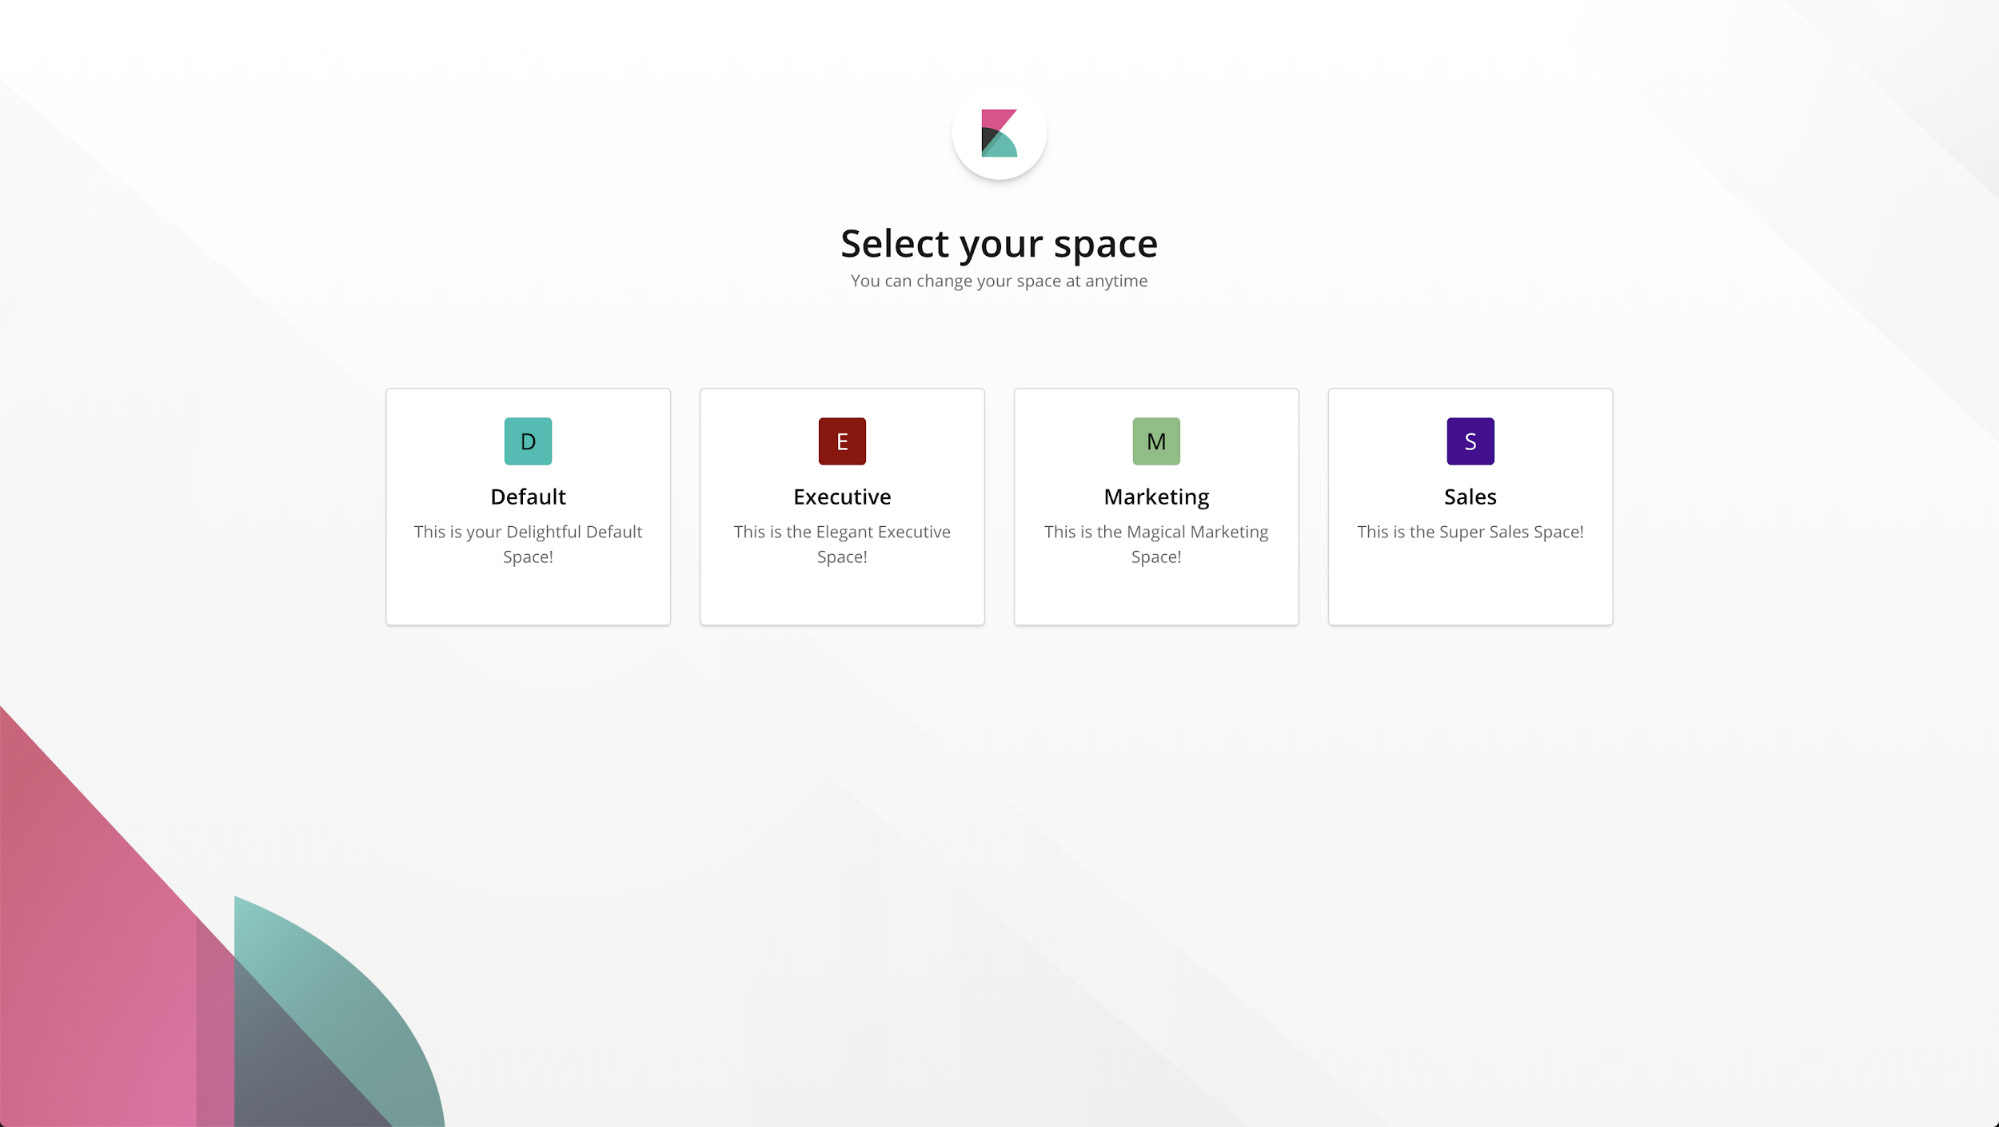
\includegraphics[width=12cm, keepaspectratio]{img/spaces_kibana.jpg}
					\caption{Selector de espacios de trabajo en Kibana.}
					\label{fig:spaces_kibana}
				\end{figure}
				
				La última versión estable de Kibana es la 7.8.0 \cite{versions_kibana}, liberada el 18 de Junio del 2020. En la versión final desarrollada se ha utilizado Kibana 7.7.0 publicada el 13 de Mayo del 2020.


				
	\chapter{INTEGRACIÓN DE MONGODB Y MATPLOTLIB EN KIBOTICS}
		En este capítulo se describe el estado inicial de Kibotics Webserver, tanto arquitectura de la aplicación como tecnologías ya utilizadas. Además, se exponen los pasos realizados para la integración de MongoDB como base de datos, y de Matplotlib como generador de visualizaciones para Kibotics Webserver.
		
		\section{Estado inicial de Kibotics Webserver}
			En esta sección se describe la arquitectura que poseía Kibotics Webserver al comienzo del desarrollo de este proyecto.
			\subsection{Arquitectura}
				Kibotics es un servicio web para docencia en robótica y programación, desarrollado en Django. El servidor está compuesto por varias partes:
				
				\begin{itemize}
					\item Kibotics Webserver: Servicio web desarrollado en Django, es el centro de Kibotics y donde se generan los logs sobre los que se trabajará en este proyecto fin de carrera.
							
					
					\item Kibotics Websim: Simulador robótico que se ejecuta unicamente en el lado del cliente. Desarrollado en A-Frame, HTML5, JavaScript, entre otras. Permite a los usuarios aprender los fundamentos de la programación robótica y visión artificial.
				\end{itemize}
				
				\textbf{(INCOMPLETO - arquitectura antigua)}
				\begin{figure}[H]
					\centering
					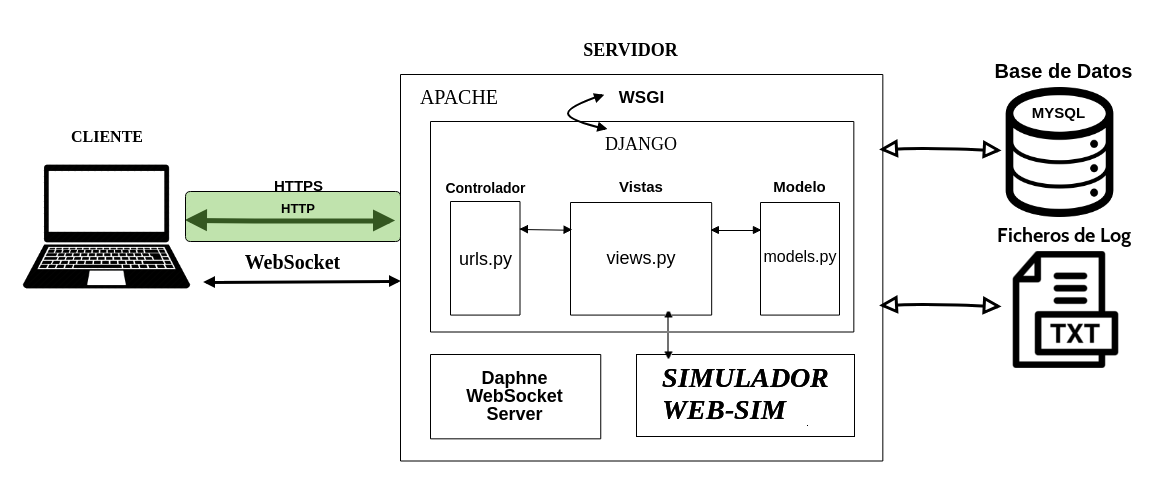
\includegraphics[width=13cm, keepaspectratio]{img/esquema_Kibotics.png}
					\caption{Arquitectura Kibotics.}
					\label{fig:arquitectura_kibotics}
				\end{figure}
			
				Cuando un usuario accede a la plataforma lo hace a través del protocolo \texttt{HTTPS} hacia el servidor Django principal. Este servidor es el orquestador de eventos que tienen lugar en el resto de máquinas.
				
				\textbf{(INCOMPLETO - arquitectura antigua)}
				\begin{figure}[H]
					\centering
					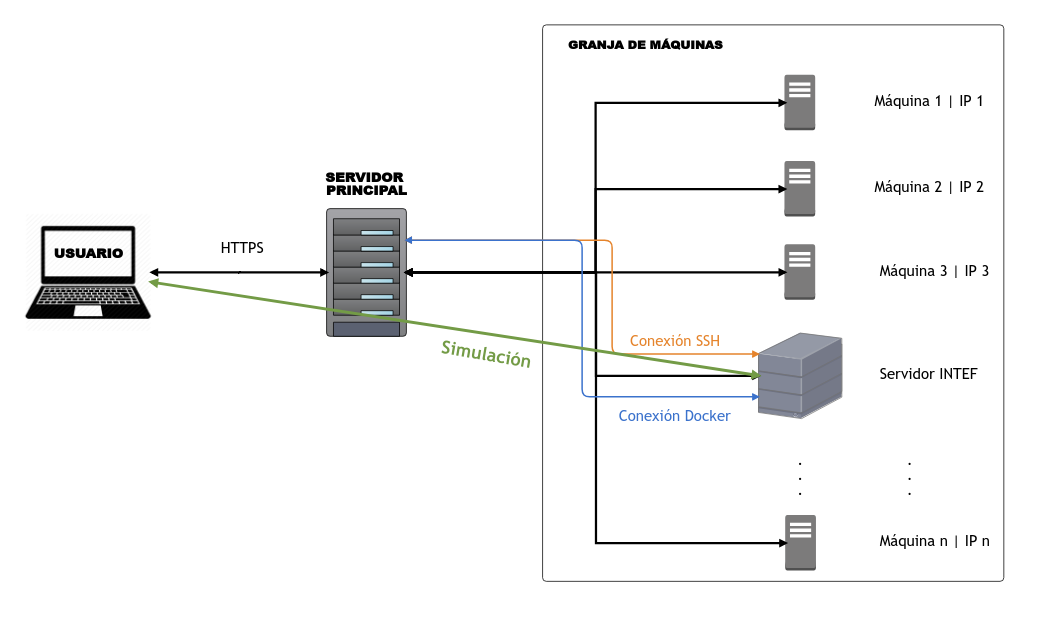
\includegraphics[width=11cm, keepaspectratio]{img/kibotics-infraestructura.png}
					\caption{Infraestructura Kibotics.}
					\label{fig:infraestructura_kibotics}
				\end{figure}
				El aspecto clave de Kibotics Webserver son las simulaciones. Una simulación está compuesta principalmente de dos partes: el código que programa el estudiante (izquierda) y la ventana de simulación (derecha), en la que el usuario verá su código ejecutado en tiempo real.

				\begin{figure}[H]
					\centering
					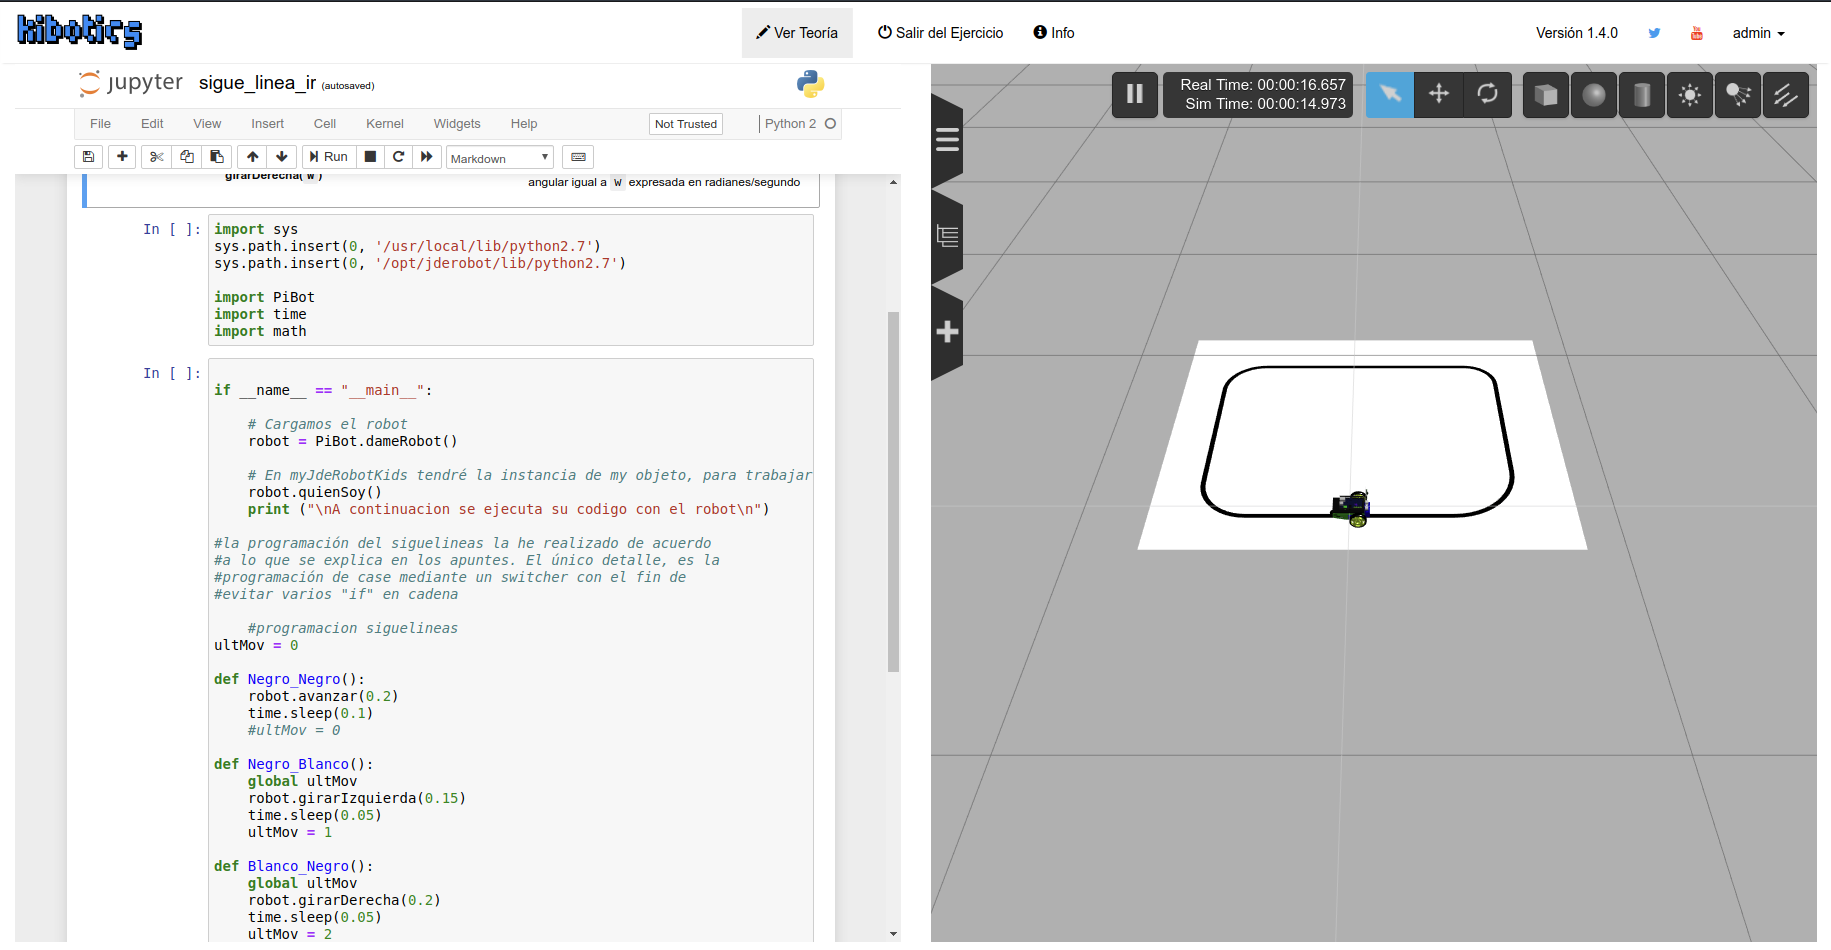
\includegraphics[width=15cm, keepaspectratio]{img/simulacion_kibotics.png}
					\caption{Simulador Kibotics.}
					\label{fig:simulacion_kibotics}
				\end{figure}

			\subsection{Logs}
			Los logs generados por la aplicación Django se guardan en una serie de archivos indexados en el servidor con formato YYYY-MM-DD-log.txt. Teniendo así, un fichero por día con todos los eventos registrados.\\
						
			Esta metodología disponía de un sistema numeral de códigos para identificar el evento que había generado cada registro de log. Cada uno de estos registros estaba separado por la cadena de caracteres: "\ |\ ".\\
			
			Estos códigos numéricos y su estructura son los siguientes:
			\begin{itemize}
				\item Log in: "1 | date | user name | user IP | HTTP\_USER\_AGENT"
				\item Log out: "2 | date | user name | user IP | HTTP\_USER\_AGENT"
				\item Comienzo ejecicio: "3 | date | user name | user IP | simulation type | exercise ID | host IP | HTTP\_USER\_AGENT"
				\item Fin ejecicio: "4 | date | user name | user IP | simulation type | exercise ID | host IP | HTTP\_USER\_AGENT"
				\item Error 500: "5 | 500 Internal Server Error"
			\end{itemize}
		
			Estos log, se generaban en el servidor Django haciendo uso de sondas Python, las cuales registran el evento en distintas partes del código del servidor para guardarlas en los ficheros. Un ejemplo de estas sondas para el registro de un evento de \textit{log in} es:
			
			\begin{Verbatim}[tabsize=4]
log = open(DIRECTORY + "/logs/" + str(date.today()) + "-log.txt", "a")

traze = "1 | " + str(datetime.now().strftime("%d/%m/%Y %H:%M:%S")) 
+ " | " + username + " | " + client\_ip  + " | " + user\_agent + "\\n"\\

log.write(traze)

log.close()	
			\end{Verbatim}
			
			Además de estos logs generados en Django, se disponía de los generados de forma automática por Apache. Apache separa los eventos registrados en dos ficheros:  
			\begin{itemize}
				\item Un archivo con la salida general de la aplicación, asociada a los prints y excepciones producidas en el servidor.
				\item Un archivo de acceso al servidor que muestra las peticiones HTTP que este ha recibido.
			\end{itemize}

			
		\section{Desarrollo local}
			En está sección se describe la evolución del método de recogida y análisis de los logs. Así como una primera prueba de concepto de la herramienta de analíticas.
			\subsection{MongoDB en Kibotics Webserver}
			Kibotics Webserver disponía de una tecnología primitiva de trazabilidad de eventos basada en ficheros TXT y con limitados eventos. Con un gran coste computacional derivado de la apertura y cierre constante de ficheros, limitaba la explotación masiva de estos datos para la generación de estadísticas útiles.\\
			
			Kibotics es una plataforma que pretende dar soporte a una gran cantidad de usuarios. Por lo tanto, se espera que la capacidad de procesamiento, almacenamiento y consulta de los logs aumente. Haciendo uso de ficheros de texto plano no se podrá conseguir la velocidad de procesamiento necesaria. \\
			
			Es por esto, por lo que en un primer prototipo se decidió cambiar a un motor de bases de datos, MongoDB, una base de datos externa a Django. A la que se realizarán consultas de Python mediante la librería pymongo. La cual ofrece las herramientas de consulta y guardado necesarias para una interacción ágil con MongoDB.\\
			
			Para realizar esta migración de tecnología, es necesario primero instalar MongoDB:
			
			\begin{Verbatim}[tabsize=4]
$ sudo apt-get install mongodb-org
			\end{Verbatim}

			
			Una vez instalado, iniciar el proceso para levantar el servicio MongoDB se puede realizar con la siguiente sentencia:
			
			\begin{Verbatim}[tabsize=4]
$ sudo systemctl start mongod
			\end{Verbatim}
			
			Adicionalmente a esto, podemos reiniciar o parar el servicio con los siguientes sentencias respectivamente:
			
			\begin{Verbatim}[tabsize=4]
$ sudo systemctl restart mongod
$ sudo systemctl stop mongod
			\end{Verbatim}
			
			Con el servicio MongoDB ya instalado lo único necesario para completar la migración de registro de logs, es modificar las sondas previamente definidas. Estas sondas, pasarán de escribir en ficheros a registrar los eventos en MongoDB.
			
			Haciendo uso de la librería pymongo la tarea se simplifica mucho. Primero, importamos la librería y abrimos la conexión con la base de datos, para ello: 
			
			\begin{Verbatim}[tabsize=4]
import pymongo
myclient = pymongo.MongoClient("mongodb://localhost:27017/")
mydb = myclient["kiboticsDDBB"]
			\end{Verbatim}
			
			Ya con las conexiones necesarias realizadas, las sondas se transforman a, por ejemplo, las de nueva sesión y simulación:
			\begin{Verbatim}[tabsize=4]
# Nueva sesión
mydict = {
	"date" : datetime_object_test, 
	"username" : "USERNAME_TEST", 
	"client_ip" : "CLIENT_IP_TEST", 
	"user_agent" : "USER_AGENT_TEST"
}
mydb["newSession"].insert_one(mydict)


# Nueva simulación
mydict = {
	"date" : datetime_object_test, 
	"username" : "USERNAME_TEST", 
	"client_ip" : "CLIENT_IP_TEST", 
	"simulation_type" : "SIMULATION_TYPE_TEST",
	"exercise_id" : "EXERCISE_ID_TEST",
	"host_ip" : "HOST_IP_TEST",
	"container_id" : "CONTAINER_ID_TEST",
	"user_agent" : "USER_AGENT_TEST"
}
mydb["newSimulation"].insert_one(mydict)
			\end{Verbatim}

			
			Con estos pasos, el registro de eventos de log en la nueva base de datos MongoDB ya está completo. para recuperar la información y tratarla en el servidor se hará uso de pymongo. Las sentencias o \textit{queries} de búsqueda para los diferentes eventos logueados serán:
		
		
			\begin{Verbatim}[tabsize=4]
# Sentencia nueva sesión
dataNSES = mydb["newSession"].find({
	"username" : {'$regex' : "USERNAME_TEST"}, 
	"date" : {'$lte': first_day_test, '$gte': last_day_test}
});

# Sentencia fin de sesión	
dataESES = mydb["endSession"].find({
	"username" : {'$regex' : "USERNAME_TEST"}, 
	"date" : {'$lte': first_day_test, '$gte': last_day_test}
});

# Sentencia nueva simulación
dataNSIM = mydb["newSimulation"].find({
	"username" : {'$regex' : "USERNAME_TEST"}, 
	"date" : {'$lte': first_day_test, '$gte': last_day_test}
});

# Sentencia fin de simulación
dataESIM = mydb["endSimulation"].find({
	"username" : {'$regex' : "USERNAME_TEST"},
	"date" : {'$lte': first_day_test, '$gte': last_day_test}
});

			\end{Verbatim}	
			
			Como se puede observar, estas sentencias de búsqueda filtran tanto por usuarios como por rangos de fechas. Esto aporta cierta flexibilidad en la obtención de los eventos logueados, evitando así tener que recorrer datos o ficheros extra descartando registros de log como se haría con la metodología de ficheros que poseía Kibotics inicialmente.
			
			\subsection{Matplotlib en Kibotics Webserver}
			Matplotlib es una librería Python de generación de visualizaciones tanto estáticas, como animadas. Haciendo uso de ella, se han generado todas las visualizaciones necesarias para el primer prototipo.\\
						
			Estas visualizaciones inicialmente se han separado en dos secciones, analíticas de simulaciones y sesiones. Ambas pueden ser filtradas tanto por usuarios como rangos de fechas.\\
			
			Siguiendo la metodología detallada en las secciones anteriores surge un problema, los datos de inicio y fin, tanto para las sesiones como para las simulaciones, están separados en distintas tablas de MongoDB. Por lo tanto, para hacer una relación entre ambos es necesario cruzarlos en Python para unificarlos en un único evento de sesión o simulación. \\
			
			Para solventar esta problemática, se desarrolló un método con esta funcionalidad de unificación de registros, con el que se consigue extraer información valiosa de duración de eventos:
			
			Este código extrae todos los usuarios contenidos en el campo \texttt{'username'} y posteriormente recorre los registros de apertura de cada uno de ellos. Buscando por el campo \texttt{'date'} de los eventos de cierre hasta encontrar la inmediatamente posterior que será almacenado junto con la duración del evento. \\
			
			Como salida del método, se devolverá un diccionario de diccionarios con cada uno de los eventos sesión/simulación para cada usuario del que haya ocurrencias.\\
			
			\begin{Verbatim}[tabsize=4]
def formatDatesUser(newData, endData):
	USERS = newData.distinct("username")
	newData.sort([('Username', -1), ('date', -1)])
	endData.sort([('Username', -1), ('date', -1)])
	Dict = {}
	
	for user in USERS:
		for d in newData:
			for dd in endData:
				if(dd['username'] == d['username'] == user):
					if(d['date']<dd['date']):
						if(user not in Dict):
							Dict[user] = {d['date'] : 
								{
									"totalTime" : dd['date']-d['date'],
									"endTime" : dd['date']
								}
							}
						else:
							Dict[user].update({d['date'] : 
								{
									"totalTime" : dd['date']-d['date'],
									"endTime": dd['date']
								}
							})
				break;
			endData.rewind()
		newData.rewind()

	return Dict
			\end{Verbatim}
						
			La clave de este diccionario serán los usuarios. El valor, será otro diccionario con las fechas de comienzo y fin del evento así como su duración. Un ejemplo de respuesta sera:
			
			\begin{Verbatim}[tabsize=4]
{
	"USERNAME_TEST_1" : {
		start_date_1 : {
			"endTime" : end_date_1,
			"totalTime" : end_date_1 - start_date_1
		},
		start_date_2 : {
			"endTime" : end_date_2,
			"totalTime" : end_date_2 - start_date_2
		},
		
		...
		start_date_N : {
			"endTime" : end_date_N,
			"totalTime" : end_date_N - start_date_N
		},
	},
	
	...
	"USERNAME_TEST_N" : {
		start_date_1 : {
			"endTime" : end_date_1,
			"totalTime" : end_date_1 - start_date_1
		},
		start_date_2 : {
			"endTime" : end_date_2,
			"totalTime" : end_date_2 - start_date_2
		},
		
		...
		start_date_N : {
			"endTime" : end_date_N,
			"totalTime" : end_date_N - start_date_N
		},
	}
}
			\end{Verbatim}
			
			Una vez se ha enriquecida la información disponible, ya se puede enviar a métodos de generación de visualizaciones. Se hace uso de la librería Matplotlib para crear diversas tipologías de visualizaciones:
			
			\begin{itemize}
				\item Primero, recorrerán los datos de entrada formateándolos a la estructura de ejes necesaria para cada una de las visualizaciones. Generalmente se compondrá de dos listas o \textit{arrays}, uno con los datos del eje-X y otro con los referentes al eje-Y. En ciertos casos como el mapa de calor, necesitaremos una matriz de datos para la correcta representación de la información.
				
				\item Segundo, se creará la visualización y se le añadirán los datos que se formatearon en el punto primero. Este es el paso en el que se explicitará qué tipo de visualización se insertará para cada caso. Junto a la primera parte, es lo que más cambiará entre métodos.
				
				\item Tercero, se ajustará el diseño de la visualización para que encaje estéticamente tanto con las otras visualizaciones generadas para la funcionalidad de analíticas, como con el diseño ya existente en la aplicación.
				
				\item Finalmente, ya generada la visualización, se guardará la figura en un objeto \texttt{BytesIO}. Este objeto de bytes, se codificará a formato \texttt{*.png} y se devolverá por la salida del método. Esta parte de los métodos de creación de visualizaciones es muy lenta, ya que el proceso de renderizado de una imagen con la calidad suficiente para ser mostrada en el servidor no es un proceso instantáneo. Será una de los motivos por el que se haga un futuro cambio de tecnologías.
			\end{itemize}
			
			Con estos objetos de imagen ya guardados, lo único que queda es devolverlos al cliente. Para ello se utilizarán las plantillas HTML enriquecidas de Django. A continuación, se muestra una sección de una de estas plantillas en las que se puede ver como se han insertado dos imágenes:
			
			\begin{Verbatim}[tabsize=4]
...	
<div class="main">
	<h2>INICIOS POR DIA DE LA SEMANA</h2>
	<hr/>
	
	<div class='left' >
		<h4>Sesiones</h4><br>
		<img src="data:image/png;base64, {{ WeekSesion }}" 
		alt="Data not loaded properly" width=500 height=auto />
	</div>
	
	<div class='right'>
		<h4>Simulaciones</h4><br>
		<img src="data:image/png;base64, {{ WeekSimulation }}" 
		alt="Data not loaded properly" width=500 height=auto />
	</div>
</div>
...
			\end{Verbatim}
			
			A continuación, se puede ver el resultado final, con unos datos de prueba, no productivos. El prototipo nos muestra información de interés acerca de la actividad en la aplicación web.\\
			
			\begin{figure}[H]
				\centering
				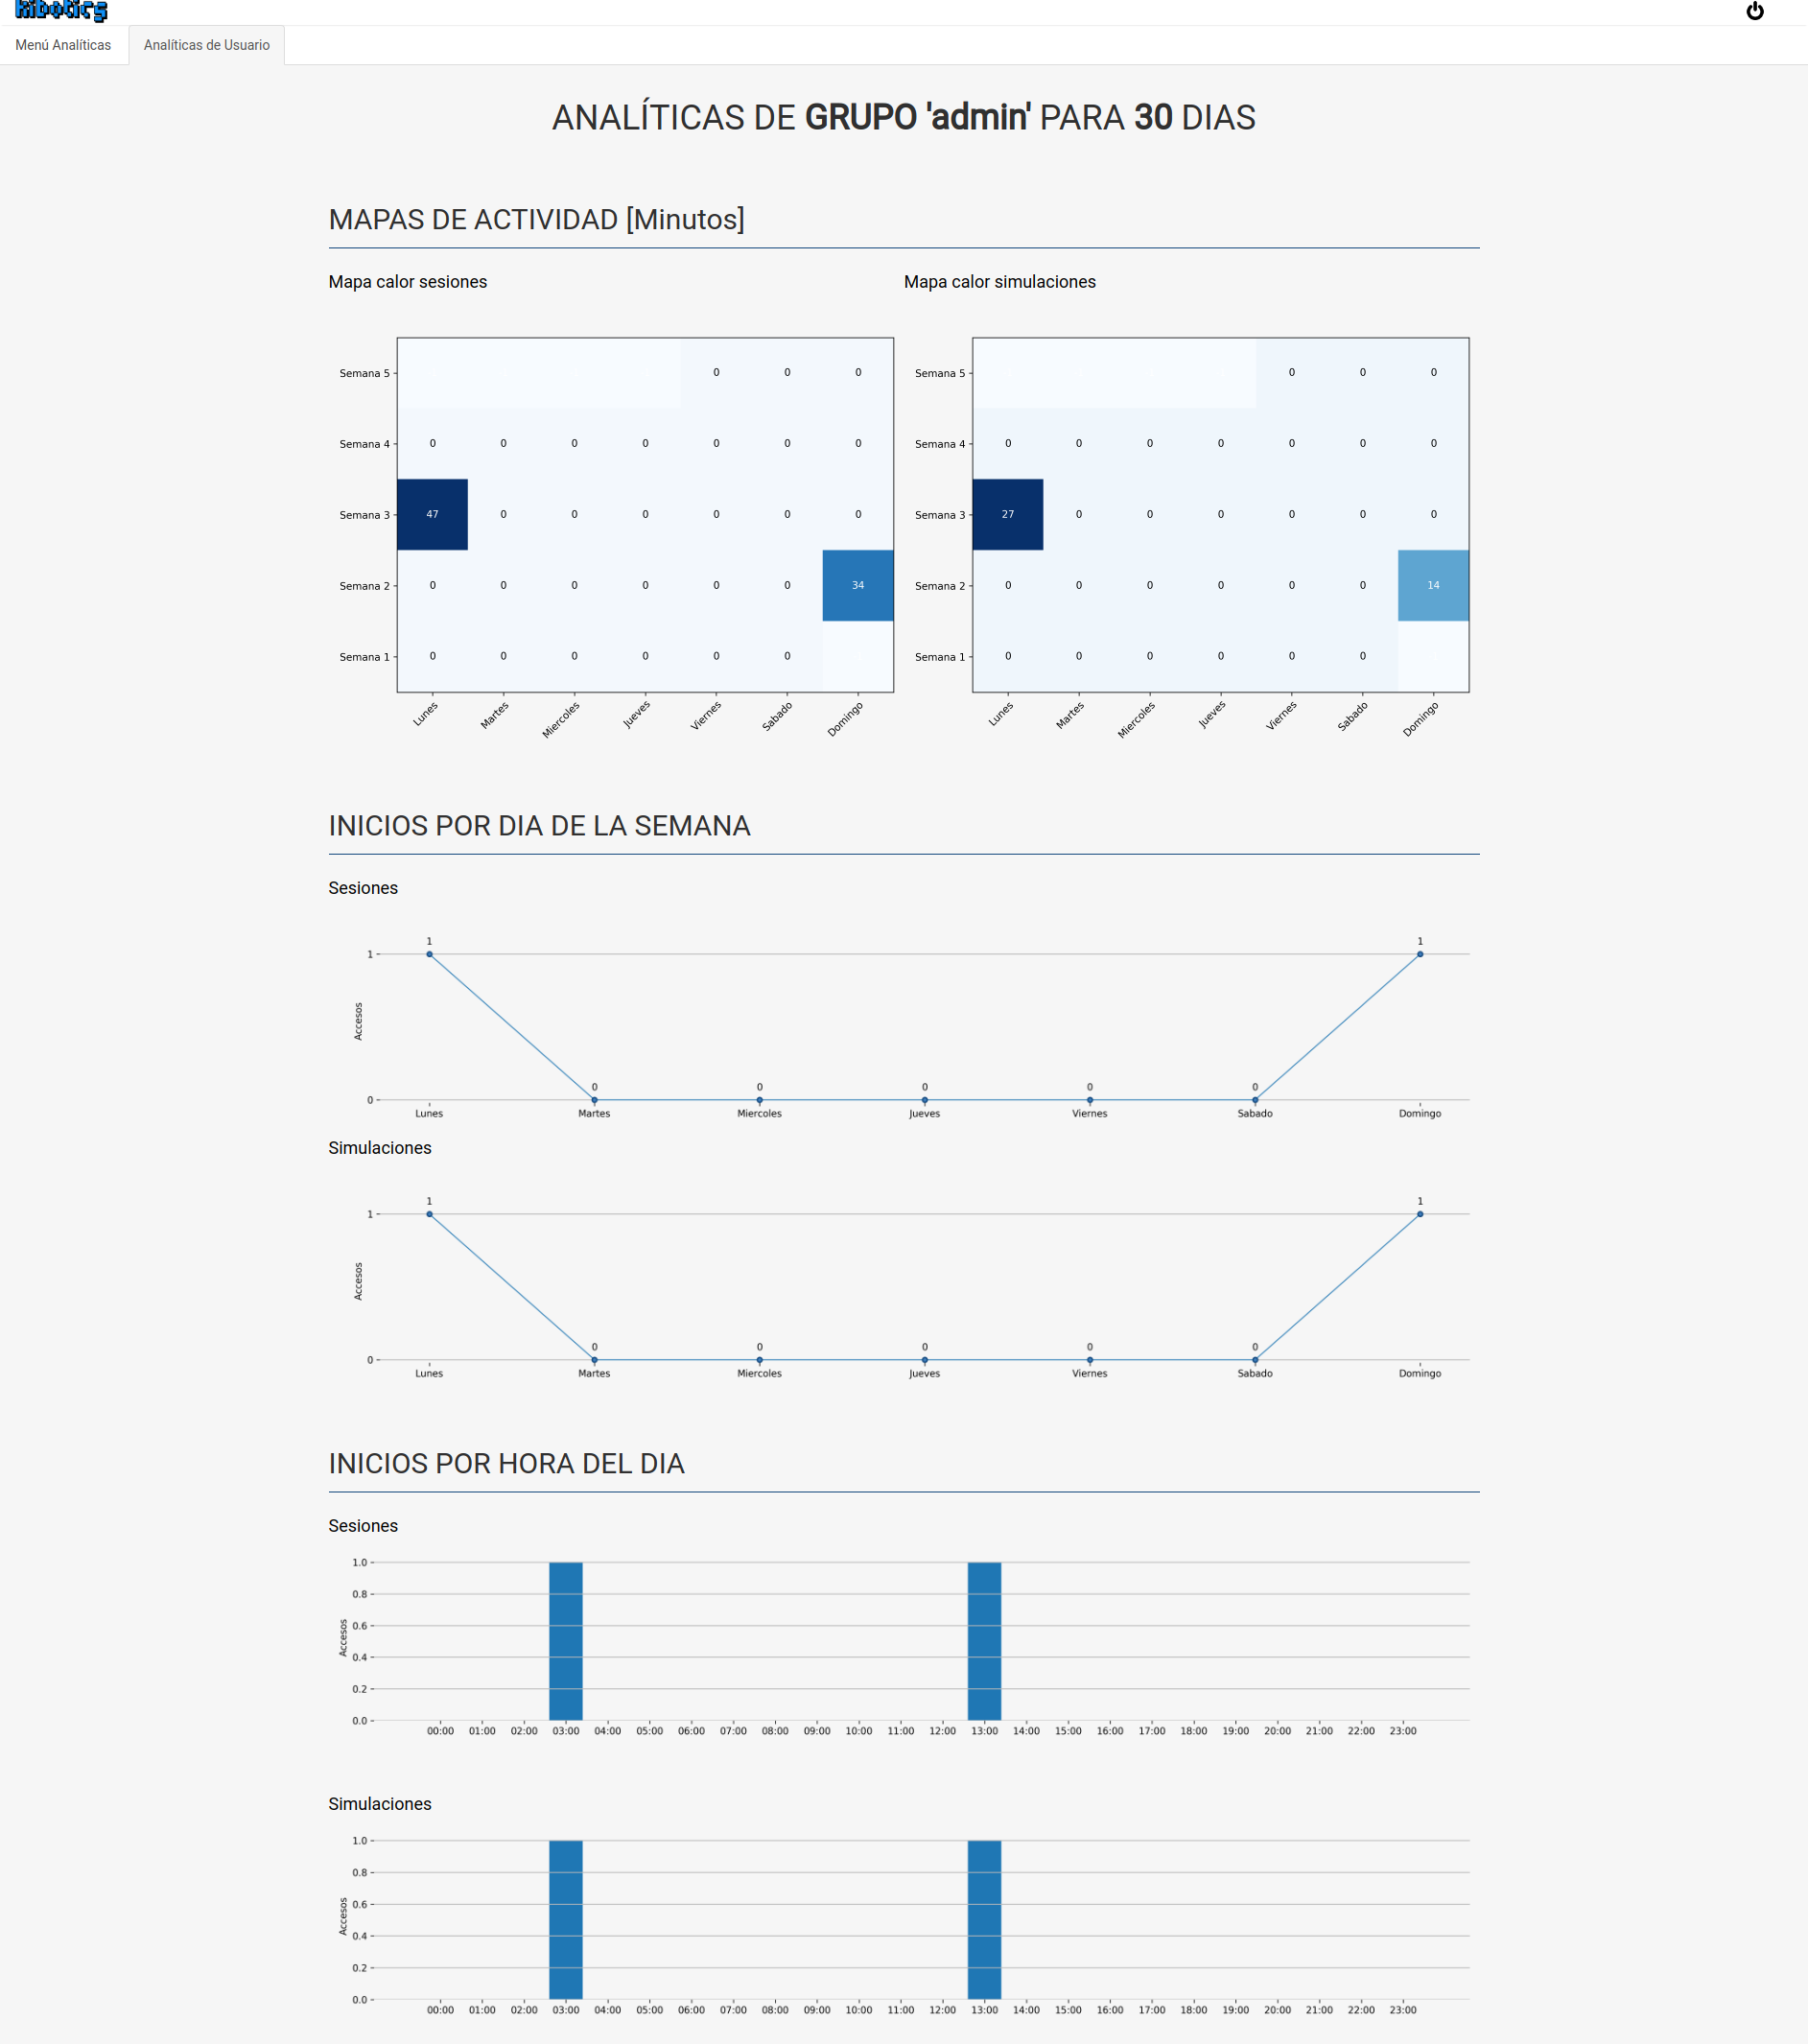
\includegraphics[width=14cm, keepaspectratio]{img/primer_prototipo_1.png}
				\caption{Primer prototipo parte 1.}
				\label{fig:primer_prototipo_1}
			\end{figure}
		
			En la primera figura, se puede observar una primera parte con dos mapas de calor, los cuales representan la actividad semana a semana (filas) en el servidor para los distintos eventos de sesión y simulación. El color será más intenso a mayor sean los minutos invertidos en ese evento para cada uno de los días (celdas).\\
			
			En una segunda parte, se representan 4 visualizaciones más con los accesos a sesiones y simulaciones separadas en dos grupos. Una primera agrupación con los accesos por día de la semana, a continuación, el segundo grupo con accesos divididos por la hora del día a la que fueron realizadas.\\
			
			En la Figura 4.5 se muestran, se representan las dos últimas secciones de este primer prototipo. Una primera sección con los tiempos totales y medios que el grupo de usuarios o usuario ha pasado en cada uno de los ejercicios a los que ha accedido. Finalmente, una última visualización que representa con un mapa geográfico la localización desde la que cada usuario ha accedido a la aplicación.\\
			
			\begin{figure}[H]
				\centering
				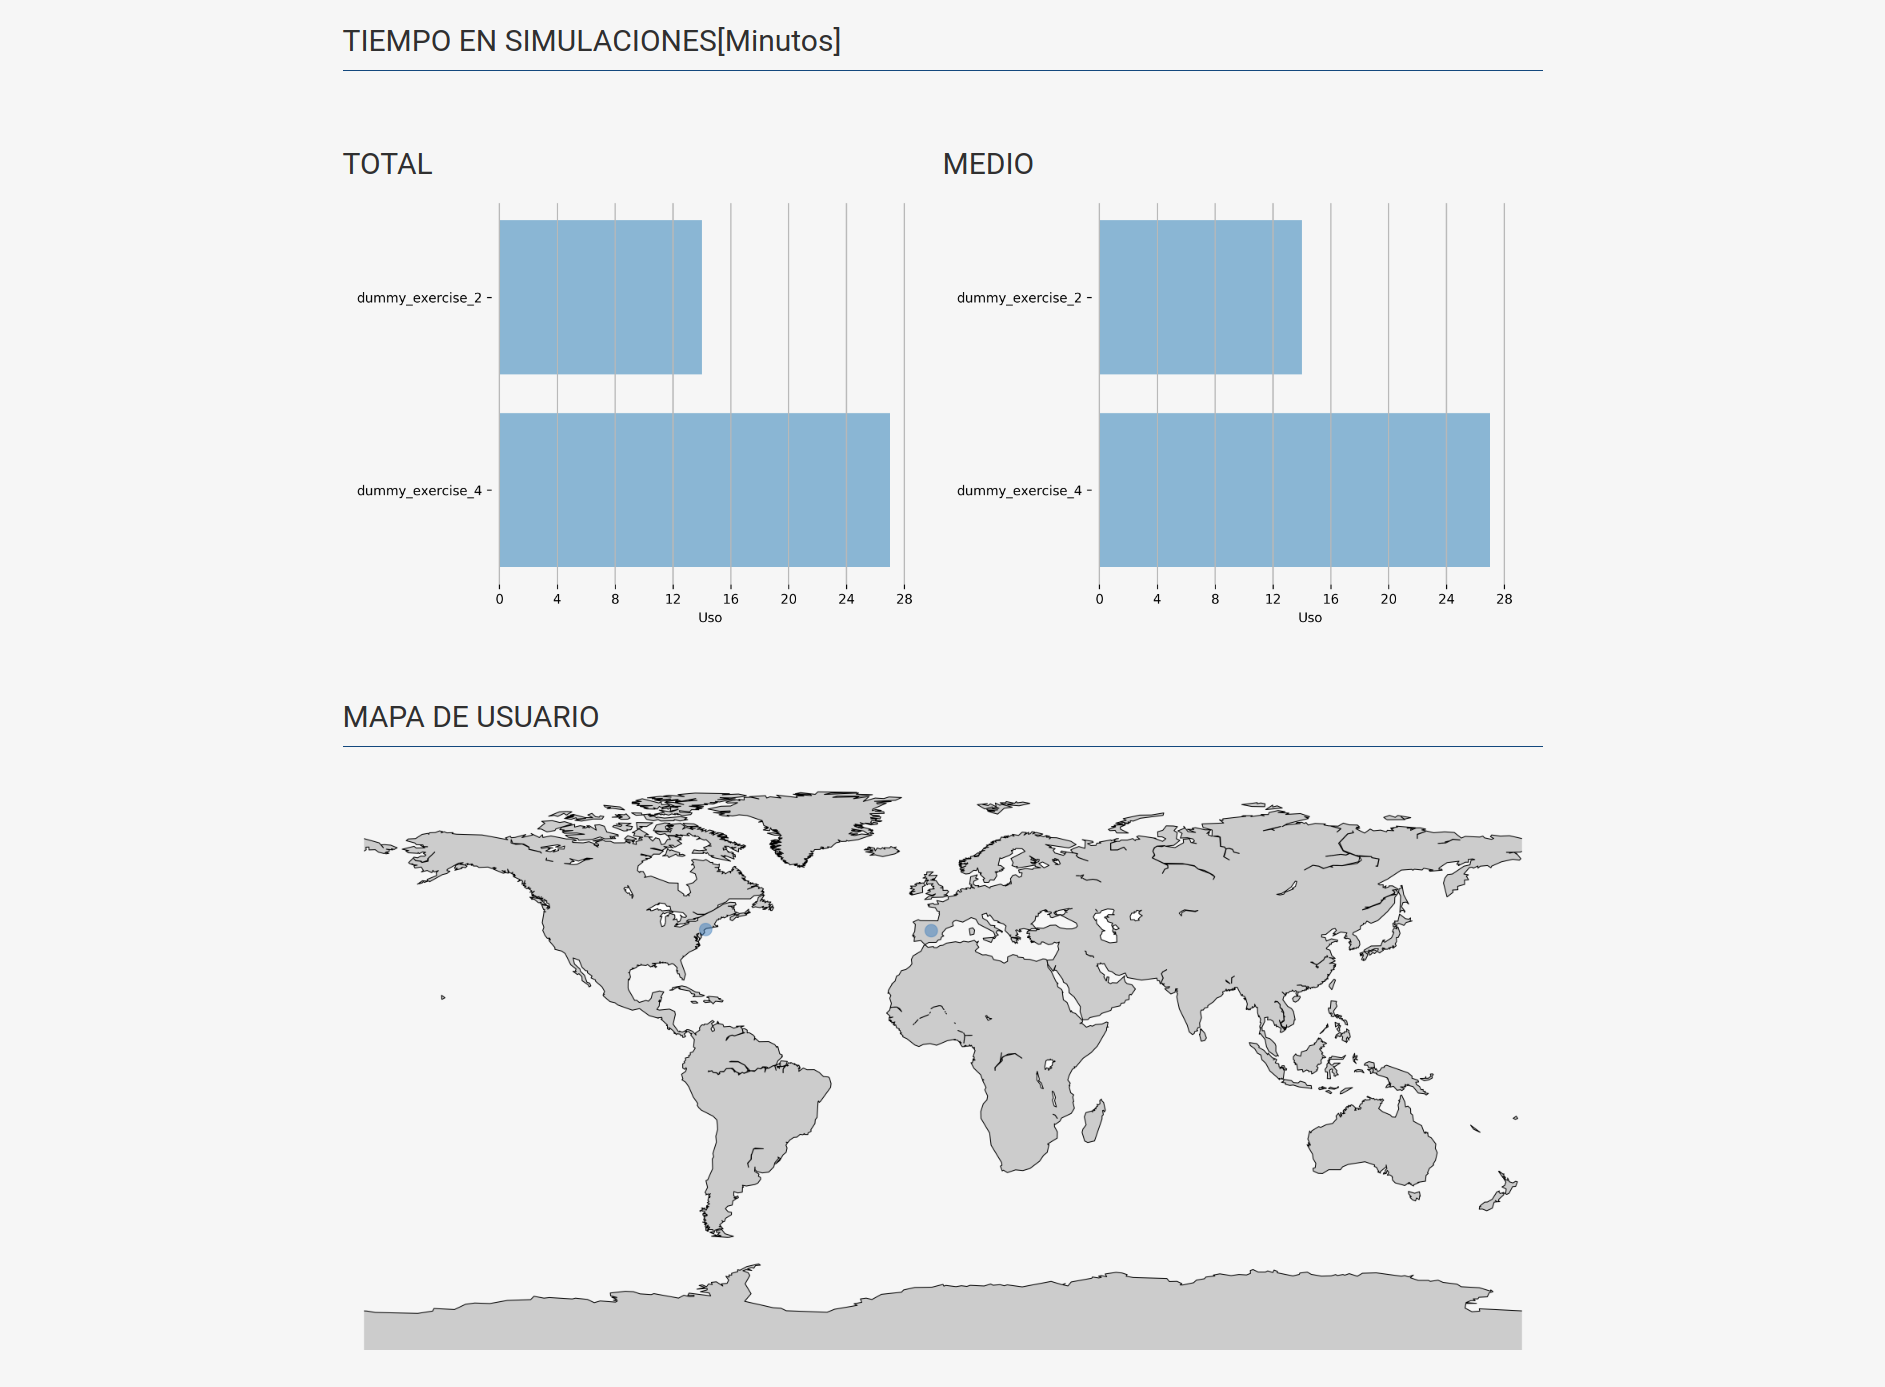
\includegraphics[width=14cm, keepaspectratio]{img/primer_prototipo_2.png}
				\caption{Primer prototipo parte 2.}
				\label{fig:primer_prototipo_2}
			\end{figure}
		
			Este primer prototipo es bastante completo pero tiene ciertos inconvenientes. Primero, falta cierta información útil que podría ser representada, como desde que dispositivos acceden los usuarios.\\
	
			Esta visualizaciones, al estar insertadas como imágenes, carecen de interactividad, la cual sería muy útil para tener información extra o poder realizar más filtrado de los datos.\\
			
			Además el módulo, al tener que renderizar cada una de las imágenes individualmente, tarda unos segundos en mostrar las visualizaciones.
		
	
	
	\chapter{INTEGRACIÓN DEL STACK ELK EN KIBOTICS}
		En este capítulo se describen las tecnologías utilizadas en la versión final desarrollada del módulo de analíticas. También se detallan una serie de instrucciones para que los futuros desarrolladores puedan integrar estas tecnologías en local.
		
		\section{Desarrollo local}
			En está sección se describe la evolución que han sufrido los logs de la aplicación. Así como la versión final de la herramienta de analíticas que hará uso del stack ELK.
			\subsection{Elasticsearch como base de datos}
				El primer paso en el proceso de migración es el cambio de base de datos, lo que obligará a modificar las sondas que almacenan estos datos de log. Para hacer uso del stack ELK, es necesario sustituir MongoDB por Elasticsearch. Para esto lo primero será instalar e iniciar un servicio de Elasticsearch en local \footnote{https://www.elastic.co/guide/en/elasticsearch/reference/current/targz.html}.\\
				
				
				Una vez iniciado el servicio Elasticsearch, ya dispondremos de la base sobre la que guardar los registros de log o documentos. Estos registros se alamcenarán en índices, cada uno de los cuales estará definido por un esquema de campos y tipologías que definirán la estructura de los documentos que se almacenen.\\
				
				Se podrán crear tantos índices como sea necesario, para consultarlos se puede lanzar una sentencia por terminal, o acceder con la IP y el puerto desde un navegador a la \texttt{API REST} configurada en instalación. Un ejemplo de llamada para un índice llamado index\_name\_test será la siguiente:
				
				\begin{Verbatim}[tabsize=4]
http://127.0.0.1:9200/index_name_test/_search/?size=1000&pretty
				\end{Verbatim}
				
				El siguiente paso en la migración es la integración de Elasticsearch en Django. Se realizará haciendo uso de la librería Python \texttt{django\_elasticsearch\_dsl}. Para migrar de MongoDB a Elasticsearch se han realizado dos pasos: creación de los índices y migración de las sondas que almacenan los logs de MongoDB a Elasticsearch.\\
				
				
				El primer paso consistió en crear los índices de Elasticsearch. Estos índices son muy similares a los modelos que se utilizan en Django para representar la información de la base de datos. Se creará los siguientes índices: 				

				\begin{itemize}
					\item \texttt{kibotics\_session\_log}: índice en el que se almacenan los eventos referentes a las sesiones.
					
					\item \texttt{kibotics\_simulation\_log}: índice en el que se almacenarán la información relativa a las simulaciones.
					
					\item \texttt{kibotics\_error\_log}: índice en el que se almacenarán los eventos referentes a los errores.
					
					\item \texttt{kibotics\_visit\_log}: índice en el que se almacenarán la información relativa a las visitas.
				\end{itemize}				
								
				Para evitar la problemática que surgió durante el desarrollo del primer prototipo, relativo al cálculo de la duración de los eventos, se ha eliminado el campo que almacenaba la fecha. Para sustituirlo, se han añadido dos nuevos campos a los índices de Elasticsearch los cuales establecerán el inicio y fin de cada evento, unificando así los dos registros de log.\\
				
				Por otro lado, el campo \texttt{USER\_AGENT}, que se almacenaba anteriormente y ofrecía información acerca del dispositivo y software que utilizaban los visiantes de la web, ha sido dividido y sustituido con la información del navegador, dispositivo y sistema operativo. Cada uno con su propio campo en los esquemas de los índices de Elasticsearch. Ofreciendo así la información de forma más clara y eliminando ciertos datos no útiles para las visualizaciones que se quieren generar.\\
				
				Para trabajar en Kibana con mapas es necesario guardar tanto la longitud como la latitud, para lo cual se hará uso de un campo ya existente llamado \textit{Geo Point} que almacenará en un diccionario ambos campos.\\
								
				Para complementar las nuevas sondas, que se han mencionado anteriormente y se explicarán con más detalle a continuación, es necesario la creación de un nuevo índice de visitas, en el que se registrarán los accesos a la pagina principal de la aplicación, estén o no registrados.\\
								
				Un ejemplo de la definición en Django del índices de sesiones de Kibotcis Webserver en el fichero \texttt{documents.py} es:
				
				\begin{Verbatim}[tabsize=4]
from django_elasticsearch_dsl import Document, Text, Date, Double, GeoPoint, Ip
				
class SessionDocument(Document):
	username = Text()
	start_date = Date()
	end_date = Date()
	duration = Double()
	client_ip = Ip()
	browser = Text()
	os = Text()
	device = Text()
	location = GeoPoint()
	
	class Index:
		name = 'kibotics_session_log'
		settings = {
			'number_of_shards': 1,
			'number_of_replicas': 0
		}		
				\end{Verbatim}
				
					
				Con todo esto, se tiene una base sólida sobre la que almacenar la información de logs, solo falta modificar el guardado en Elasticsearch, migar las sondas que almacenan los registros de log.\\
				
			 	Para enriquecer las sondas ya existentes y hacer uso de los nuevos campos e índices creados, se han añadido nuevas sondas para almacenar eventos de visitantes, así como sondas para optimizar la monitorización de salida de sesiones y simulaciones y evitar no tener un registro de inicio sin su correspondiente registro de fin de evento por un cierre busco de la aplicación o inactividad.\\
			 				 					
				Las sondas de inicio de los eventos son similares a las que se tenían anteriormente en MongoDB, un ejemlo para la sonda de inicio de simulación es:
				
				\begin{Verbatim}[tabsize=4]
SimulationDocument(
	username = "USERNAME_TEST",
	start_date = start_date_object_test,
	end_date = start_date_object_test,
	duration = 0.0,
	client_ip = "CLIENT_IP_TEST",
	simulation_type = "SIMULATION_TYPE_TEST",
	exercise_id = "EXERCISE_ID_TEST",
	browser = "BROWSER_TEST",
	os = "OS_TEST",
	device = "DEVICE_TEST",
	location = {'lat': latitude_double_test, 'lon': longitude_double_test}
).save()
				\end{Verbatim}

				Sin embargo, las sondas de fin de sesión/simulación cambian. Tendrán que buscar en Elasticsearch el último registro de log no finalizado en el índice para el usuario del cual se quiera cerrar el evento y sustituir tanto los campos \texttt{end\_date} como \texttt{duration}. \\
				
				Esto se realiza gracias al identificador que cada documento indexado posee al cual se le realiza una operación update con los nuevos campos. Un ejemplo de cierre de sesión será:
				
				\begin{Verbatim}[tabsize=4]
# Búsqueda del ultimo registro de sesión no cerrado
latest_session = Search(index="kibotics_session_log*") \
	.query("match", username=username) \
	.query('match', duration=0) \
	.sort({"start_date": {'order': 'desc'}})[0]

# Actualización de los campos end_date y duration
for hit in latest_session:
	duration = datetime.now() - datetime.strptime( \
									hit.start_date, \
	 								"%Y-%m-%dT%H:%M:%S.%f")
	 
	Elasticsearch(settings.ELASTICSEARCH_DSL['default']['hosts']) \
	.update(index = 'kibotics_session_log', 
			id = hit.meta.id,
			body = {"doc": {
						'end_date' : datetime.now(), 
						'duration' : duration.total_seconds()
					}
				}
			)
				\end{Verbatim}
				
				Durante el desarrollo de está lógica es útil hacer uso de la interfaz de Elasticseach para comprobar que todos estos campos están siendo creados y actualizados correctamente. A la que se accederá mediante la \texttt{URL} y puerto configurados durante el proceso de instalación.\\
				
				En esta \texttt{API}, podremos realizar filtrados por campos e índices haciendo uso de expresiones regulares \textit{Regex}, por ejemplo para acceder al índice en el que se almacenan los documentos relativos a los logs de sesiones, podremos acceder mediante la siguiente \texttt{URL}:
				
				\begin{Verbatim}[tabsize=4]	
http://127.0.0.1:9200/kibotics_session_log/_search/?size=1000&pretty
				\end{Verbatim}

				En la siguiente figura se puede observar la respuesta que se obtiene de la API de Elasticsearch en el navegador a la llamada anterior.
					
				\begin{figure}[H]
					\centering
					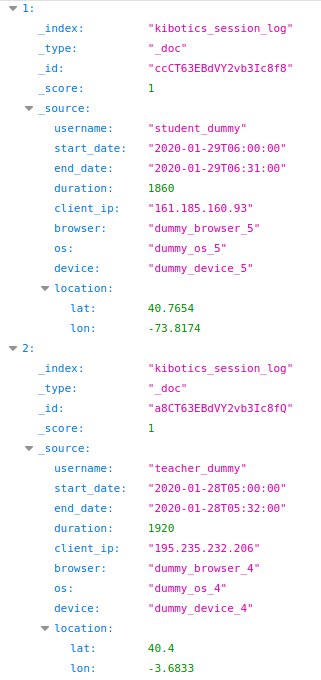
\includegraphics[width=6cm, keepaspectratio]{img/api_elasticsearch.png}
					\caption{API Rest Elasticsearch.}
					\label{fig:api_elasticsearch}
				\end{figure}

			\subsection{Kibana en Kibotics Webserver}
				
				Para acceder a Kibana, deberemos primero instalar y ejecutar el servicio\footnote{https://www.elastic.co/guide/en/kibana/current/targz.html}. Una vez Kibana está ejecutando podremos acceder a su interfaz gráfica mediante la URL y puerto configurado en la instalación:
				
				\begin{Verbatim}[tabsize=4]	
http://127.0.0.1:5601/app/kibana#/home
				\end{Verbatim}
				
				Ya con datos en Elasticsearch, Kibana nos pedirá que añadamos los índices sobre los que queremos obtener soporte y seleccionemos el campo sobre el que se filtrarán temporalmente estos logs. En este caso, el campo start\_date.

				\begin{figure}[H]
					\centering
					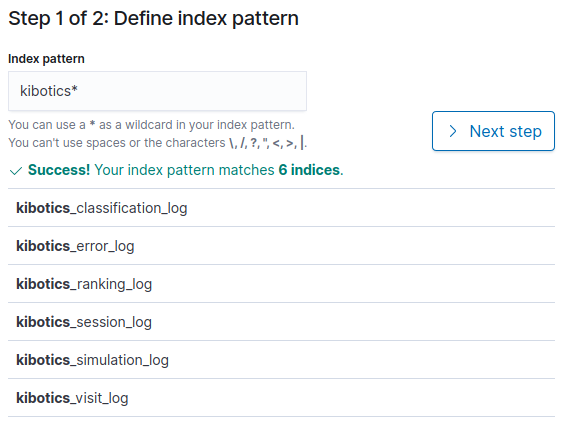
\includegraphics[width=11cm, keepaspectratio]{img/index_pattern_kibana.png}
					\caption{Creación de índices en Kibana.}
					\label{fig:index_pattern_kibana}
				\end{figure}
			
				Configurados todos los índices en Kibana, se podrá tener una primera visualización de los documentos indexados en Elasticsearch en la pestaña \textit{Discover} de Kibana. En esta pestaña podremos ver todos los logs que estén guardados, así como un histograma en el que se podrá ver gráficamente la evolución de los índices en el tiempo. Además, esta sección \textit{Discover} proporciona la posibilidad de filtrar por rangos de fechas y campos así como se tenía en el primer prototipo de este proyecto.\\
				
				Esta sección ya nos da una primera pincelada de la potencia de procesamiento de Kibana, así como la sencillez de implementación y despliegue. Las consultas son instantáneas, notablemente más rápidas que las realizadas en el primer prototipo desarrollado.\\
				
				\begin{figure}[H]
					\centering
					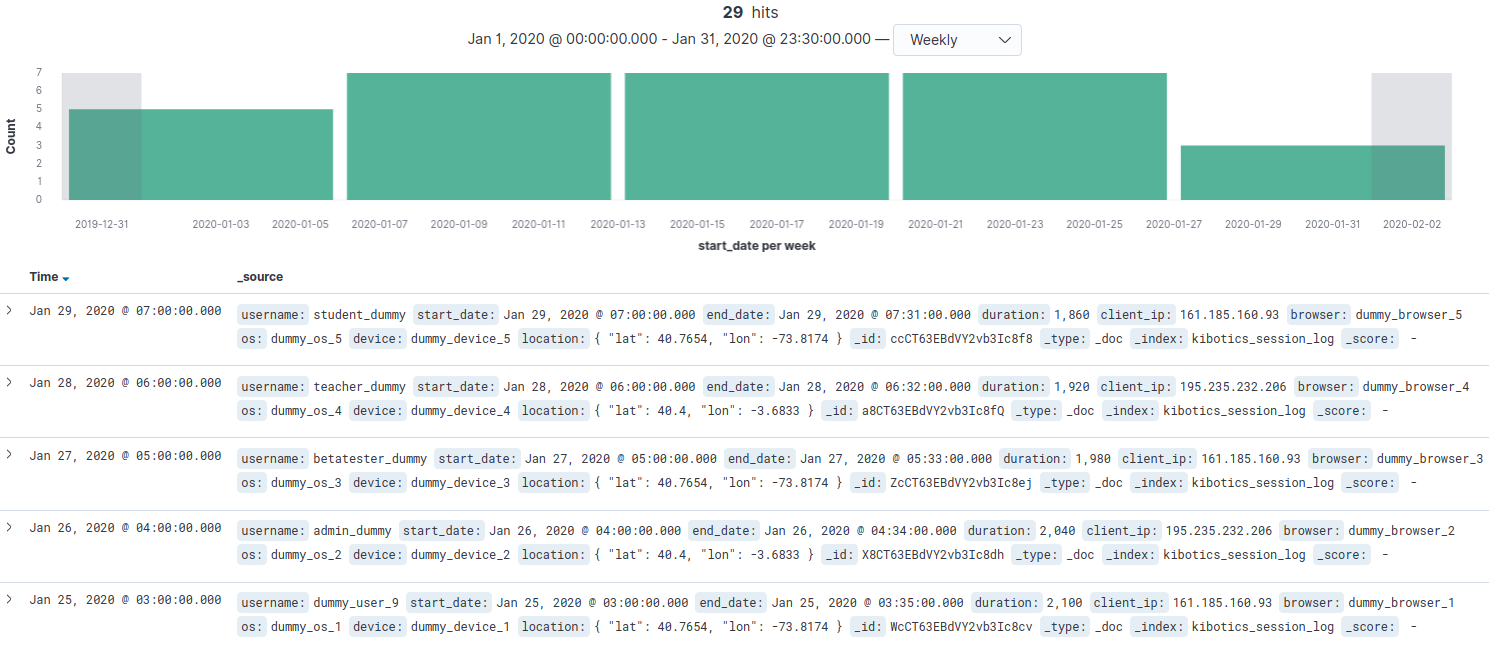
\includegraphics[width=15cm, keepaspectratio]{img/discover_kibana.png}
					\caption{Sección Discover en Kibana.}
					\label{fig:discover_kibana}
				\end{figure}
			
				Kibana ofrece la posibilidad de creación de \textit{scripted fields}, campos cuyo valor deriva de otros campos o datos ya indexados. Generados en un lenguaje muy similar a C llamado painless. \\
								
				Para el módulo de analíticas que se quiere desarrollar, y en especial para las visualizaciones que filtran por día de la semana y por hora del día, se han creado dos \textit{scripted fields} para cada uno de los índices utilizados. Estos son \texttt{day\_of\_week} y \texttt{hour\_of\_day}, el código painless utilizado para la creación de estos campos es el siguiente:
				
				\begin{Verbatim}[tabsize=4]	
// day_of_week
["", "1 Lunes", "2 Martes", "3 Miercoles", "4 Jueves", "5 Viernes",
 "6 Sabado", "7 Domingo"] [doc['start_date'].value.dayOfWeek]

// hour_of_day
doc['start_date'].value.hourOfDay
				\end{Verbatim}
				
				Con estos \textit{scripted fields} además de los almacenados en los documentos, Kibana ya dispone de todos los datos necesarios para la creación de las visualizaciones. Para ello, en la sección \textit{Visualize}, Kibana tiene una colección de distintas plantillas gráficas. Estas plantillas serán las que se configuren con los índices, documentos y campos a usar para la generación de los distintos tipos de visualizaciones.
				
				\begin{figure}[H]
					\centering
					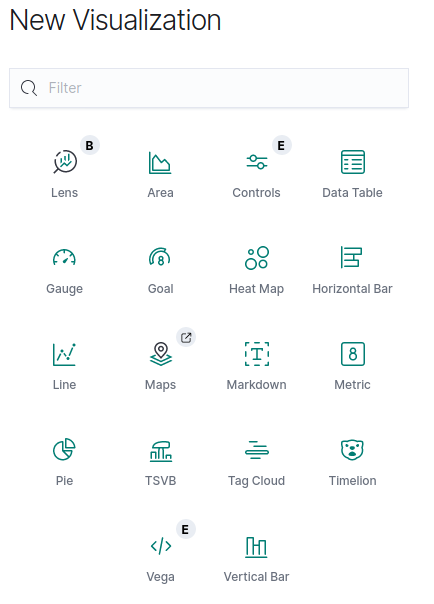
\includegraphics[width=5cm, keepaspectratio]{img/visualization_selector.png}
					\caption{Menú creación de visualizaciones.}
					\label{fig:visualization_selector}
				\end{figure}
			
				Para esta versión final del módulo de analíticas, se han creado una amplia selección de visualizaciones de las que obtener información de actividad de los usuarios. Divididas en dos \textit{Dashboards} o tableros, el primero reservado a los visitantes no registrados y el segundo para analíticas de sesiones y simulaciones de usuarios registrados. A continuación, se mostrarán las visualizaciones creadas así como una explicación de lo que representan.\\
				
				BORRARBORRARBORRARBORRAR BORRARBORRARBORRARBORRARBOR RARBORRA RBORRARBORRARBOR RARBORRARBORRARBORRARBORRARBORRARBOR RARBORRA RBORRARBORRARBORRARBORRARB ORRARBORRARBORRARBORRARBORRARBORR   ARBORRARBORRARBORRARBORRARBORRARBORRARBORRARBORRARBO RRARBOR R ARBORRARBORRARBORRARBORRARBO RRARBORRARBORRARBORRARBORRARBO RR ARBORRARBORRARBORRARBORRAR BORRARBORRARBORRARBORRARBORRARB ORR ARBORRARBORRARBORRARBORRARBORR ARBORRARBORRARBORRARBORRAR
				BORR   ARBORRARBORRARBORRARBORRARBORR ARBORRARBORRARBORRARBORRARB O RRAR BORRARBORRARBORRARBORRARBORRARB ORRARBORRARBORRARBORRAR BO RRAR BORRARBORRARBORRARBORRARBOR RARBORRARBORRARBORRARBORRA
				RBORRAR BORRARBORRARBORRARBORRARB ORRARBORRARBORRARBORRARBORR
				BORRARBO  RRARBORRARBORRARBORRARBO RRARBORRARBORRARBORRARBORRA
				RBORRARBOR RARBORRARBORRARBORRARBOR RARBORRARBORRARBORRARBORR BORRARBORRA RBORRARBORRARBORRARBORRARBORRARBORRA RBORRARBORRA
				RBORRARBORRA
				
				Para tener un control del número de accesos a lo largo del tiempo se creó el histograma representado en la figura \ref{fig:kibana_histogram}. Este histograma muestra los eventos almacenados en el índice \texttt{kibotics\_session\_log} dividido día a día en el eje de abscisas.	
				\begin{figure}[H]
					\centering
					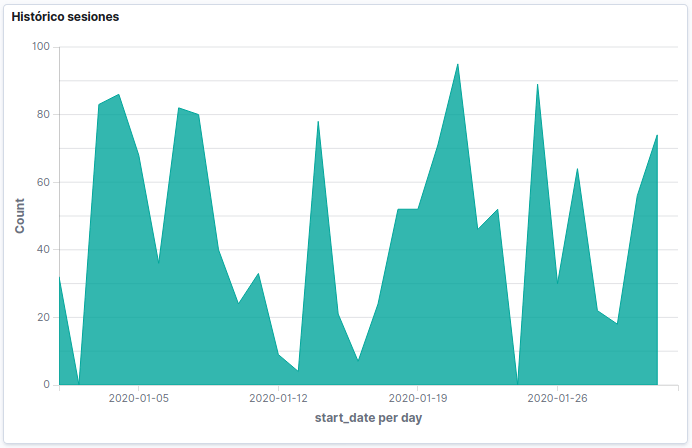
\includegraphics[width=9cm, keepaspectratio]{img/kibana_01_histogram}
					\caption{Histograma}
					\label{fig:kibana_histogram}
				\end{figure}

				Se ha creado un mapa de calor, que al igual que el histograma antes mencionado, representa la actividad de inicio de eventos. Dividido en columnas, cada una representa una semana con sus 7 días correspondientes. Un color más oscuro en la celda indica mayor actividad para ese día. Como se puede observar en la figura \ref{fig:kibana_heatmap}, hay una visualización para las sesiones y otro para las simulaciones, división recurrente que se observa en distintas secciones del módulo Kibana desarrollado.
				\begin{figure}[H]
					\centering
					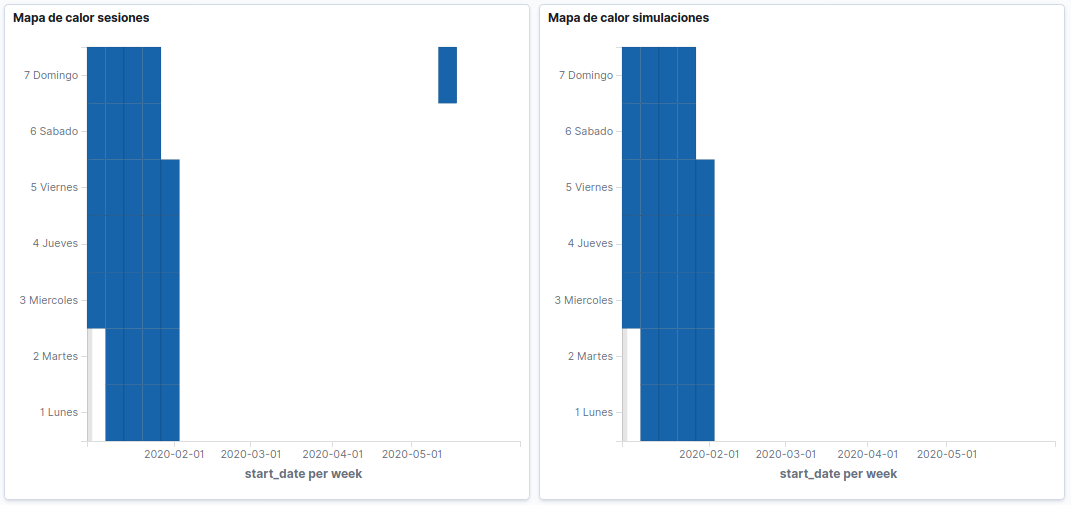
\includegraphics[width=13cm, keepaspectratio]{img/kibana_02_heatMap}
					\caption{Mapa de calor sesiones y simulaciones}
					\label{fig:kibana_heatmap}
				\end{figure}

				La siguiente figura \ref{fig:kibana_dayofweek}, dividida en dos visualizaciones, representa la actividad tanto de sesiones como de simulaciones almacenada en los índices \texttt{kibotics\_session\_log} y \texttt{kibotics\_simulation\_log} respectivamente. En formato gráfico de barras vertical, los datos, filtrados por el día de la semana en que se registraron en el campo inicio de evento \texttt{start\_date}. \\
				
				\begin{figure}[H]
					\centering
					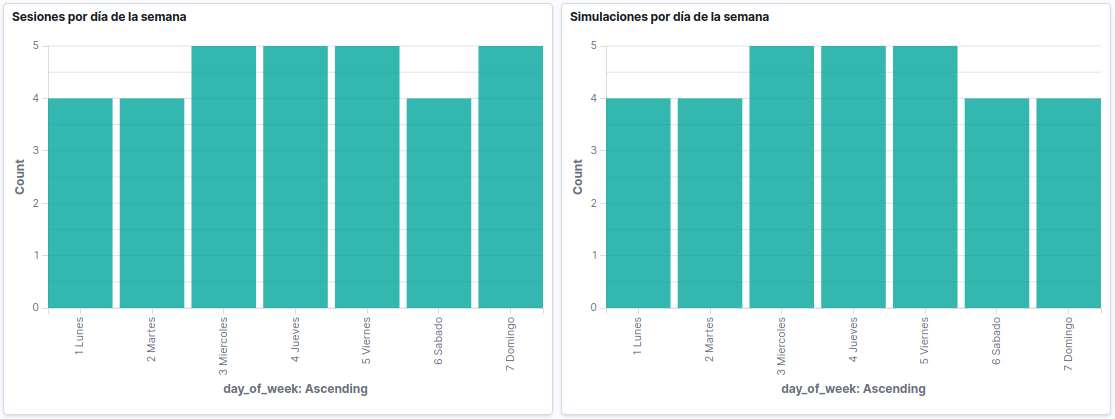
\includegraphics[width=14cm, keepaspectratio]{img/kibana_03_day_of_week}
					\caption{Gráfico de barras por día de la semana}
					\label{fig:kibana_dayofweek}
				\end{figure}

				En la figura \ref{fig:kibana_hourofday} se muestra, en dos visualizaciones con gráficas de barras verticales, la actividad en el servicio web Kibotics. Filtrados, esta vez, por la hora del día en que se registraron los eventos. Como se puede observar, cada una de estas visualizaciones corresponde a uno de los eventos que han sido logueados en Elasticsearch y almacenados en los índices \texttt{kibotics\_session\_log} y \texttt{kibotics\_simulation\_log}.\\
				
				\begin{figure}[H]
					\centering
					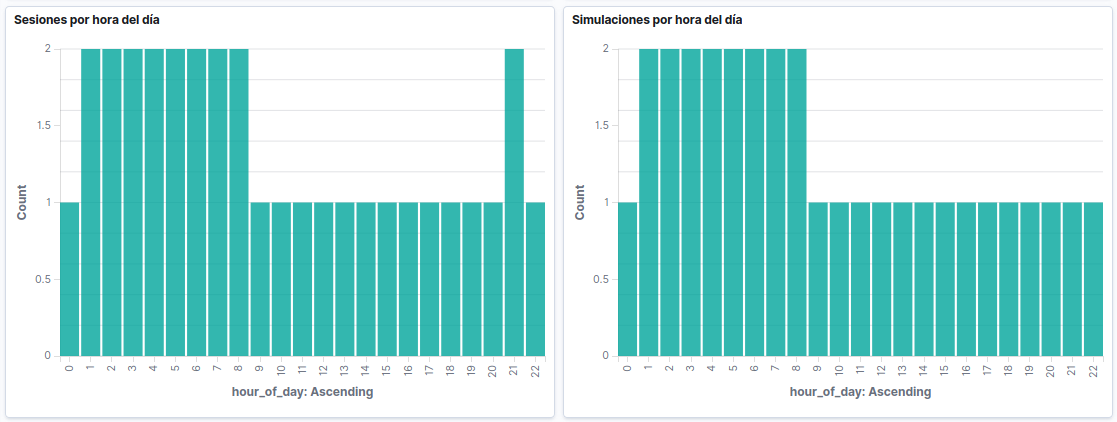
\includegraphics[width=14cm, keepaspectratio]{img/kibana_04_hour_of_day}
					\caption{Gráfico de barras por hora del día}
					\label{fig:kibana_hourofday}
				\end{figure}
\newpage		
				
				Para mostrar la actividad en las simulaciones que Kibotics ofrece, se han desarrollado las visualizaciones representadas en la figura \ref{fig:kibana_simulations}. Dividido en dos gráficas de barras que representan el tiempo invertido por los usuarios. Esta información está almacenada en el campo \texttt{duration} del índice \texttt{kibotics\_simulation\_log}. La primera visualización muestra el tiempo total invertido y la última representa el tiempo medio invertido.
				\begin{figure}[H]
					\centering
					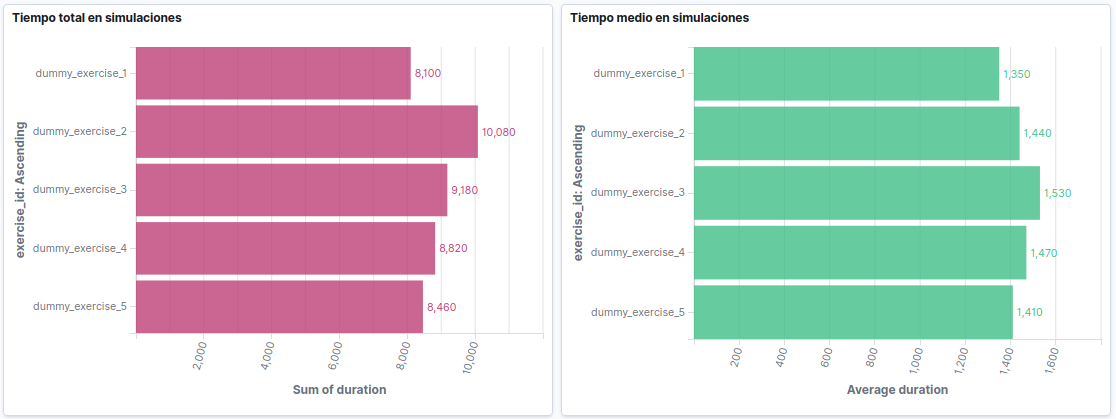
\includegraphics[width=13cm, keepaspectratio]{img/kibana_05_simulations}
					\caption{Gráfico de barras para tiempo total y medio en simulaciones}
					\label{fig:kibana_simulations}
				\end{figure}

				En la figura \ref{fig:kibana_map}, se representa gráficamente la superficie terrestre, en ella se muestran eventos de inicio de sesión ocurridos para el rango de fechas seleccionado. Hace uso de los datos de latitud y longitud almacenados en formato \texttt{Geo Point} del índice \texttt{kibotics\_session\_log}.
				\begin{figure}[H]
					\centering
					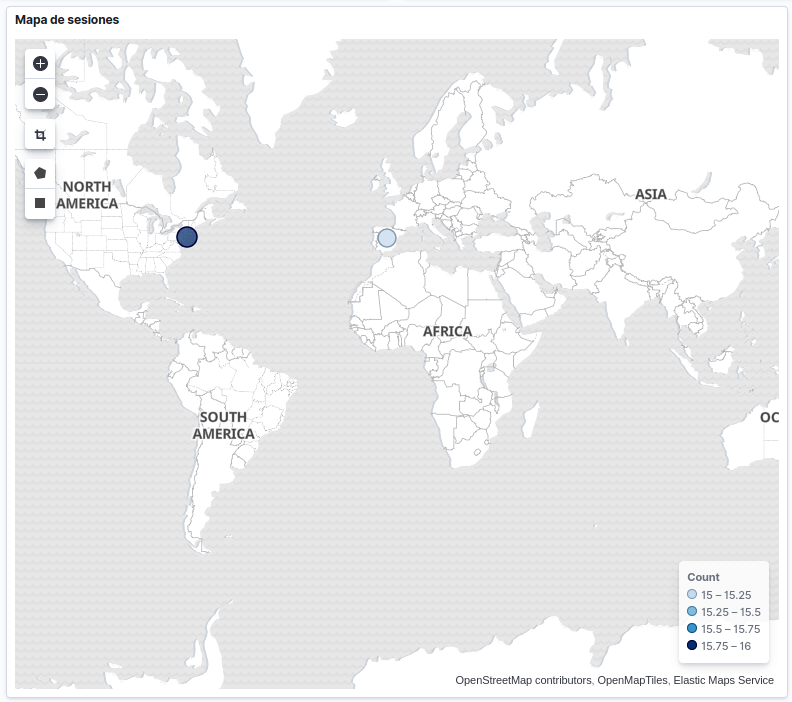
\includegraphics[width=9cm, keepaspectratio]{img/kibana_06_map}
					\caption{Mapa geográfico de sesiones}
					\label{fig:kibana_map}
				\end{figure}

				Para monitorizar el \textit{hardware} de los usuarios de la web, se han desarrollado las tres gráficas circulares mostradas a continuación en la figura \ref{fig:kibana_pie}. Cada una de ellas representa porcentualmente campos almacenados en el índice de sesiones  \texttt{kibotics\_session\_log} que proporcionan información acerca del sistema operativo, dispositivo y navegador utilizados.
				\begin{figure}[H]
					\centering
					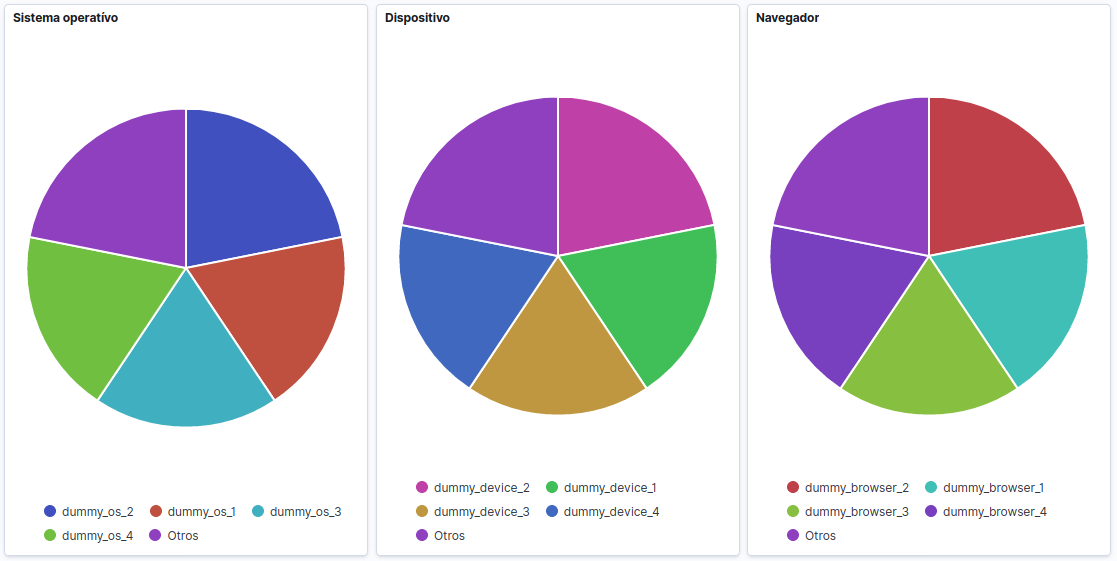
\includegraphics[width=13cm, keepaspectratio]{img/kibana_07_pie}
					\caption{Gráficas circulares para SO, Dispositivo y Navegador}
					\label{fig:kibana_pie}
				\end{figure}

				En la figura \ref{fig:kibana_latestevent}, se muestra una última sección con dos tablas de datos con los últimos eventos de sesión y simulación almacenados en los índices \texttt{kibotics\_session\_log} y \texttt{kibotics\_simulation\_log} de Elasticsearch para cada uno de los usuarios filtrados. 
				\begin{figure}[H]
					\centering
					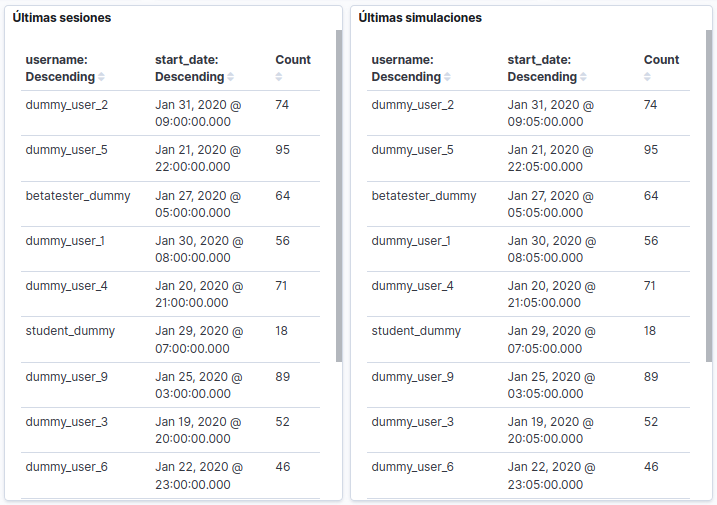
\includegraphics[width=9cm, keepaspectratio]{img/kibana_08_latest_event}
					\caption{Últimos eventos logueados}
					\label{fig:kibana_latestevent}
				\end{figure}

				
				Todas estas visualizaciones son interactivas y se puede filtrar por sus campos simplemente pulsando sobre ellas. Funcionalidad muy útil que no poseían las imágenes renderizadas que se generaban en el primer prototipo. Además, cada una de las visualizaciones del módulo desarrollado tiene una opción para ver los datos representados en texto plano e incluso descargarlos en formato \texttt{CSV} para su posterior tratamiento.\\
					
				Se han mostrado las visualizaciones referentes a la sección de sesiones y simulaciones de usuarios registrados ya que es la que más información proporciona, pero hay otra sección de analíticas de visitantes con unas visualizaciones de monitorización similares a las mostradas anteriormente.
				
				Ya creadas las visualizaciones, solo quedará integrarlas en Kibotics sustituyendo las generadas en Matplotlib. Para ello se creará una vista "menú" simple con la que se seleccionará a que tipo de analíticas se quiere acceder. Este menú selector de analíticas es el mostrado a continuación en la figura \ref{fig:kibotics_analytics_menu}.

				\begin{figure}[H]
					\centering
					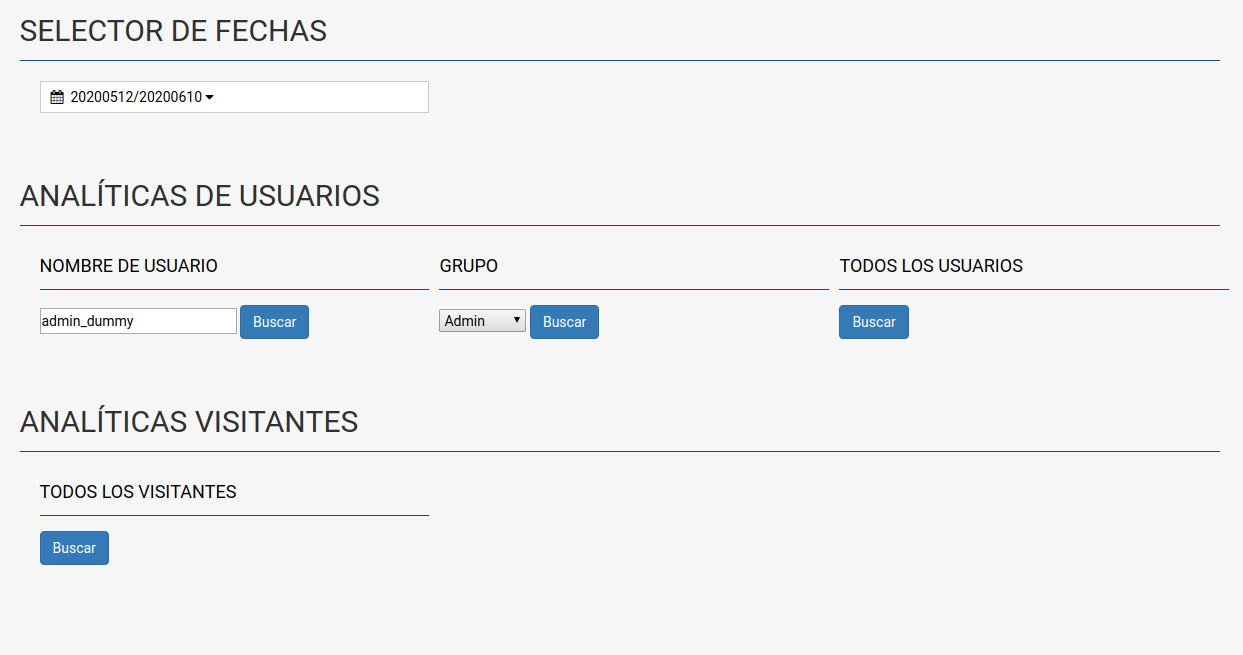
\includegraphics[width=14cm, keepaspectratio]{img/kibotics_analytics_menu.png}
					\caption{Menú de selección de analíticas en Kibotics}
					\label{fig:kibotics_analytics_menu}
				\end{figure}
			
				En esta vista se filtrará tanto por usuarios y grupos, como por fechas de las cuales se quieren analíticas. Una vez filtrado, Django generará automáticamente una URL con los datos seleccionados en el Menú de Kibotics. Esta URL dinámica apuntará a las visualizaciones de nuestro servicio de Kibana y será devuelta por el contexto de Django hasta las plantillas Django que lo insertarán en un elemento HTML iFrame. A continuación, en las siguientes figuras, se muetra Kibana ya integrado en el servicio web Kibotics.
					
				\begin{figure}[H]
					\centering
					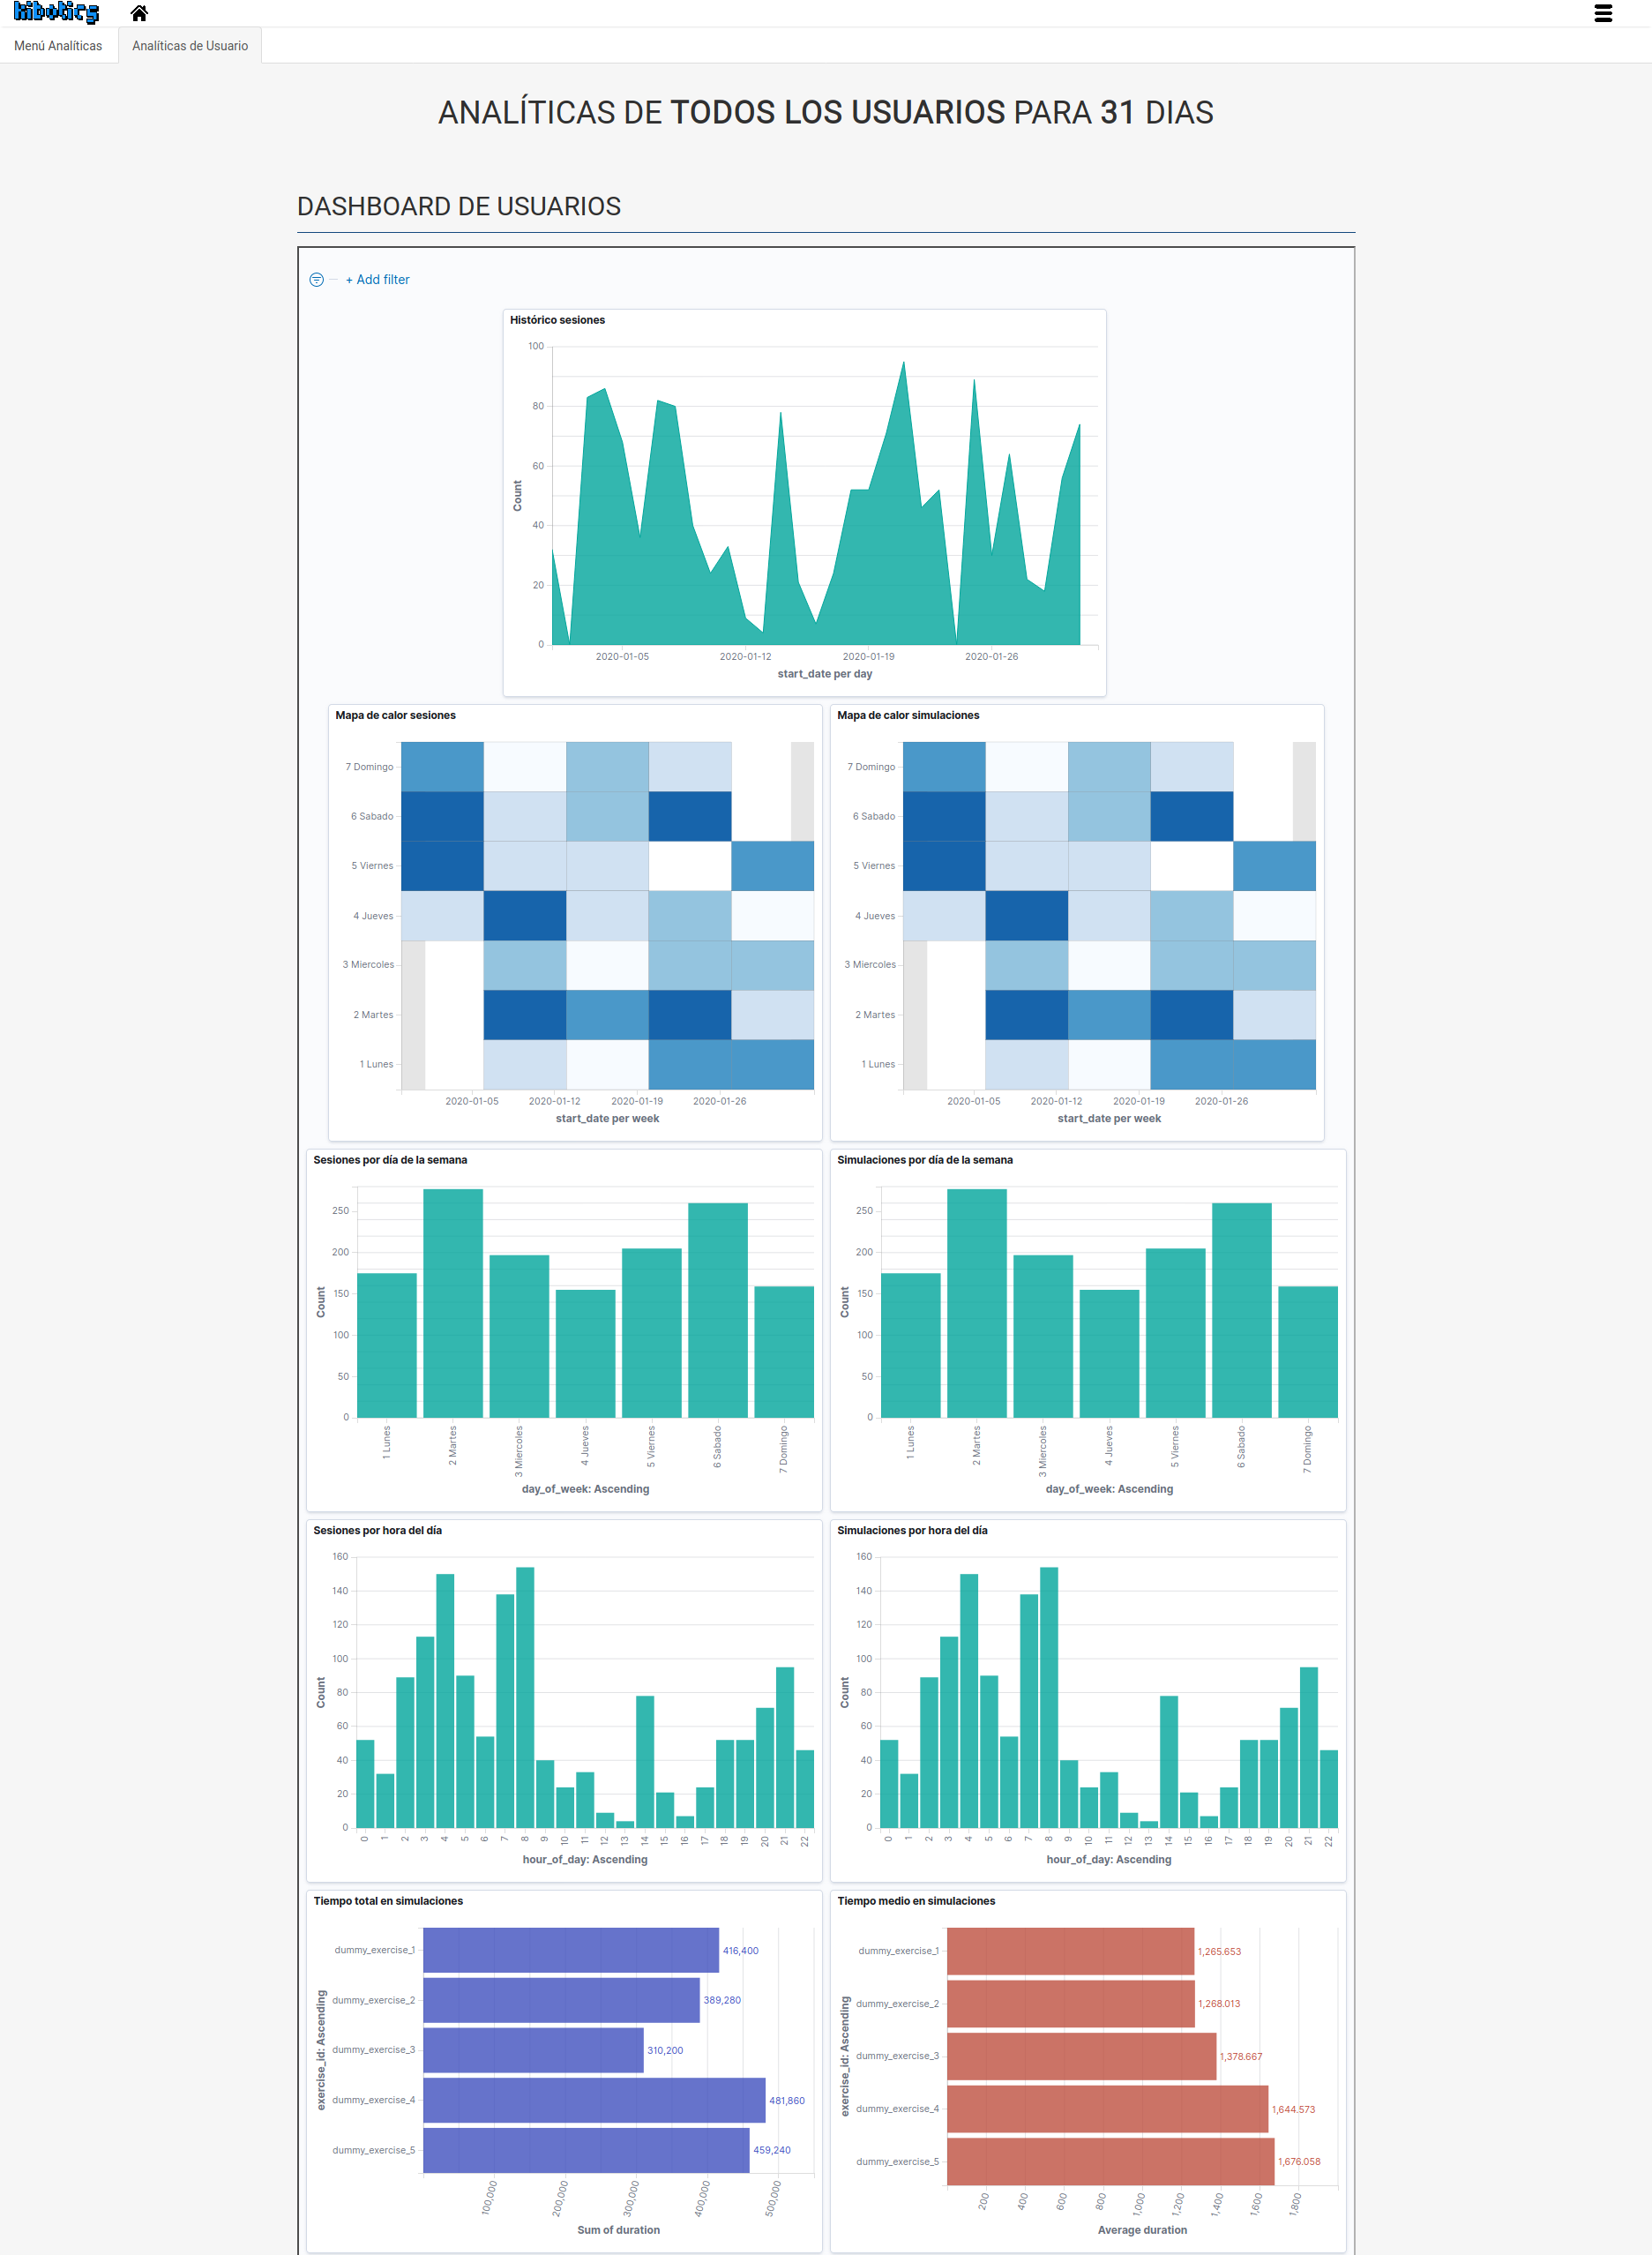
\includegraphics[width=10cm, keepaspectratio]{img/kibana_kibotics_01.png}
					\caption{Kibana en Kibotics parte 1}
					\label{fig:kibana_kibotics_01}
				\end{figure}
				\begin{figure}[H]
					\centering
					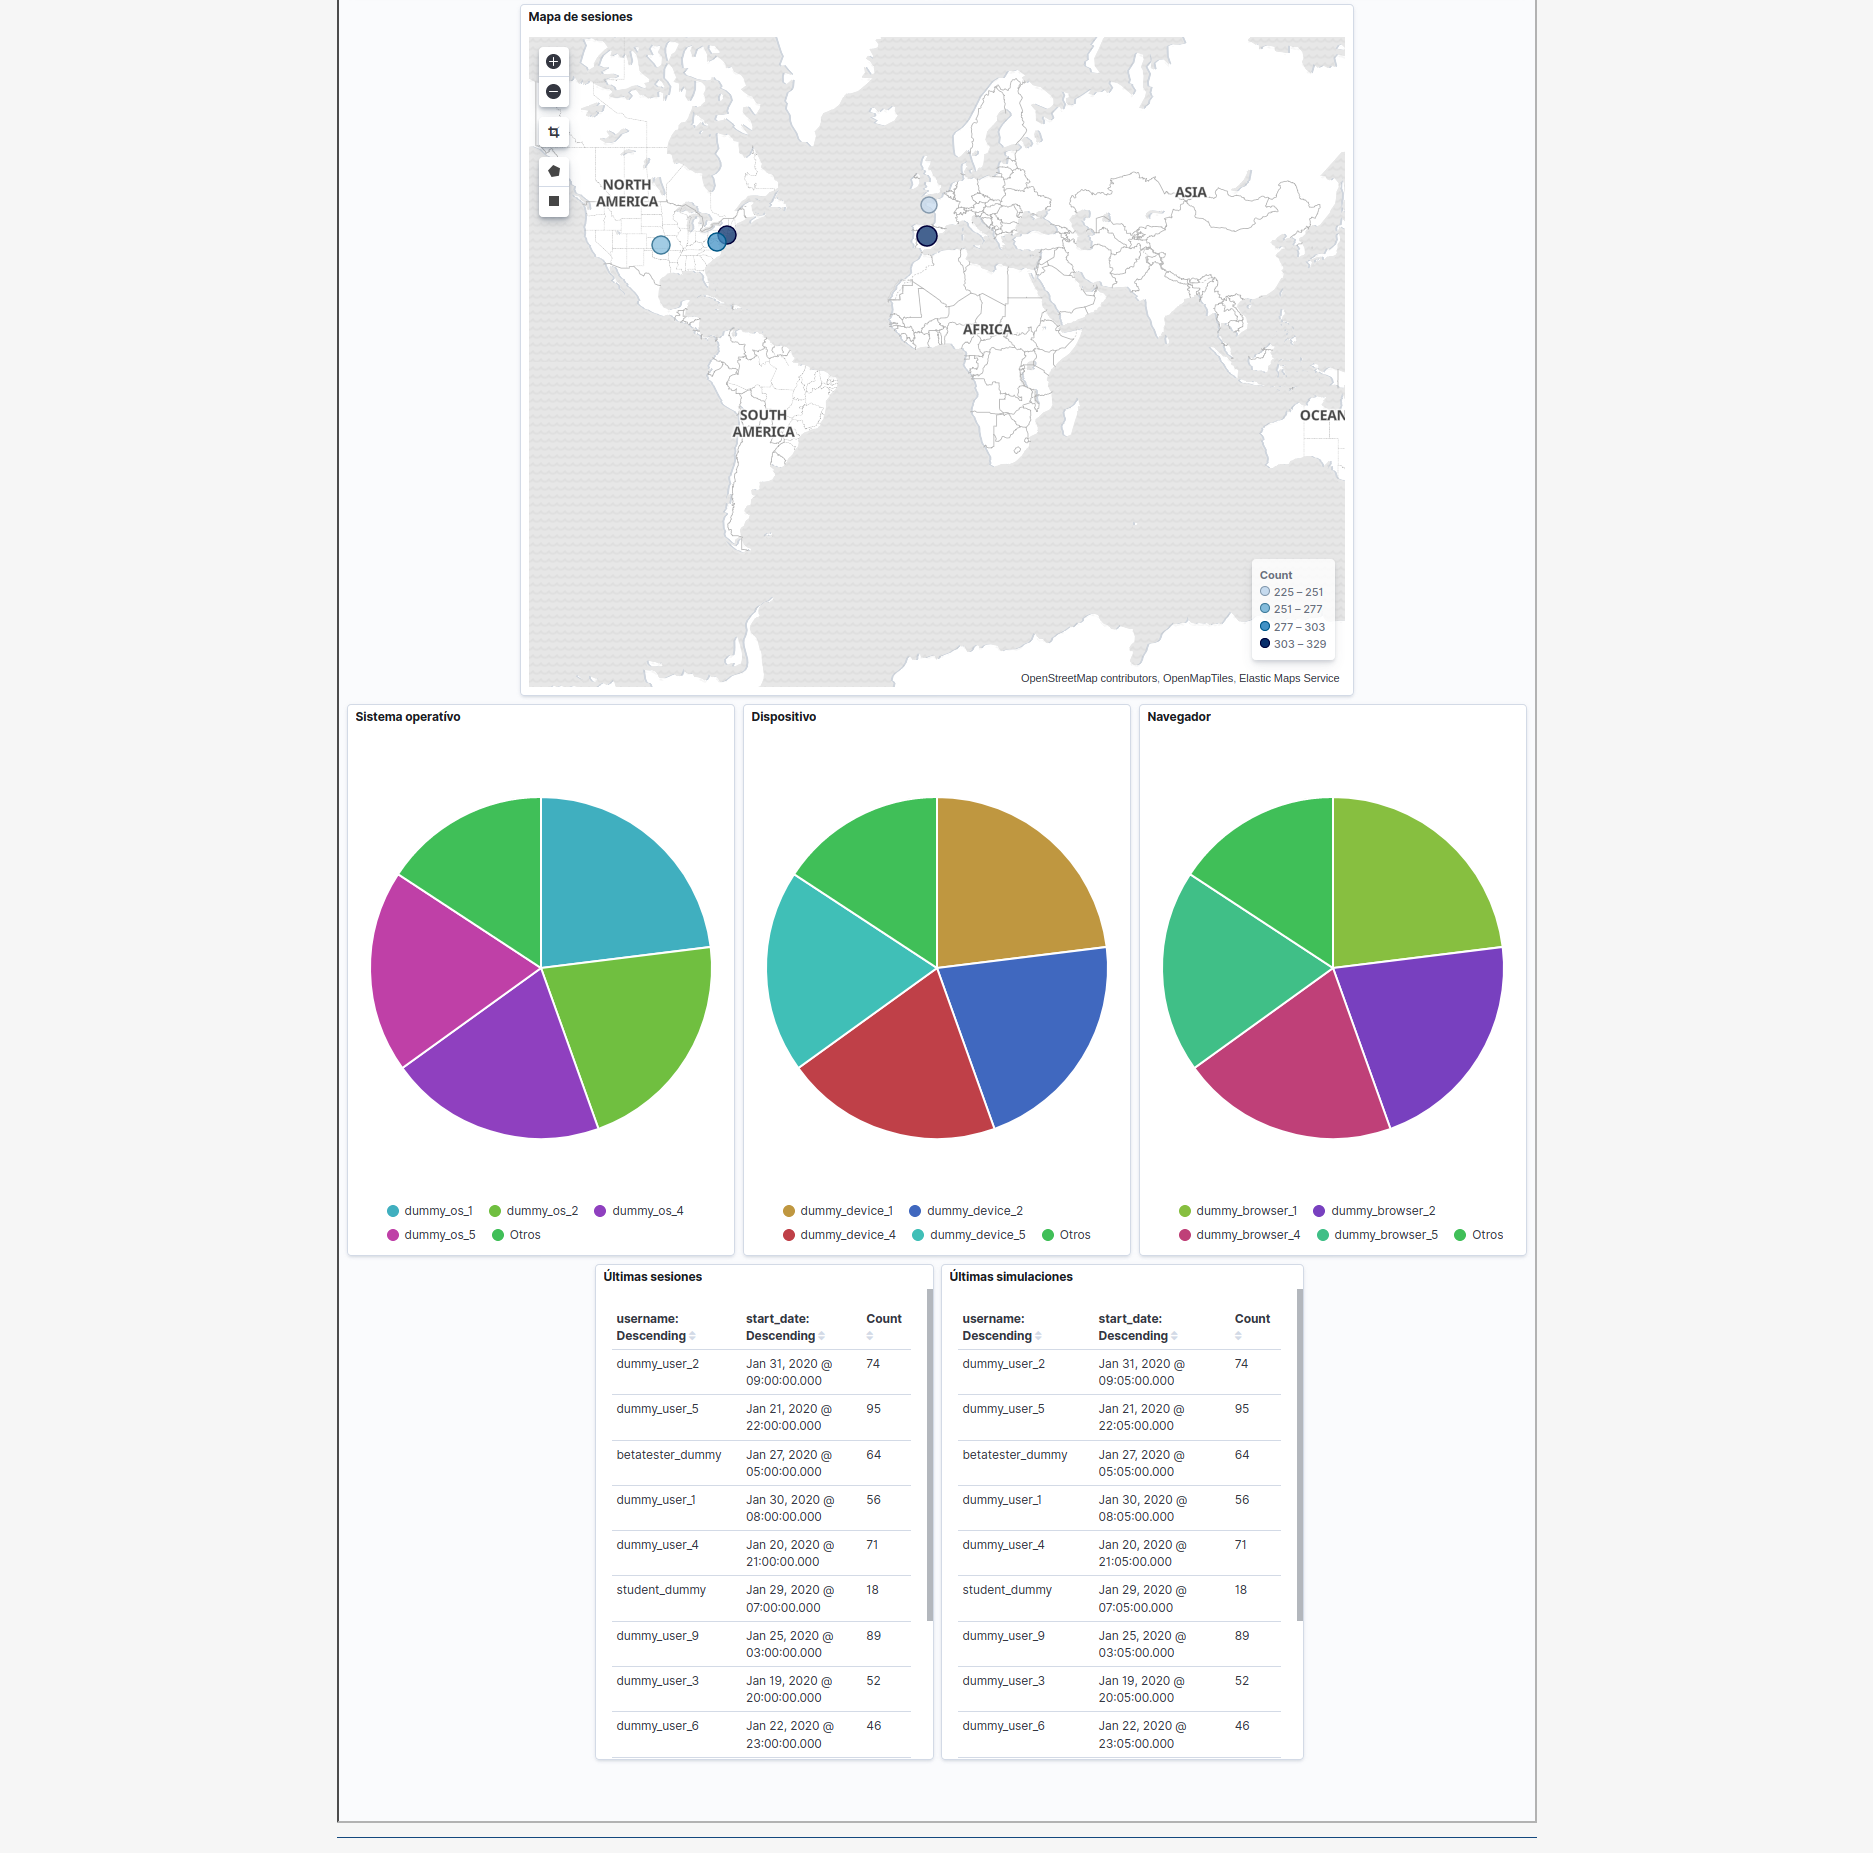
\includegraphics[width=10cm, keepaspectratio]{img/kibana_kibotics_02.png}
					\caption{Kibana en Kibotics parte 2}
					\label{fig:kibana_kibotics_02}
				\end{figure}
				\begin{figure}[H]
					\centering
					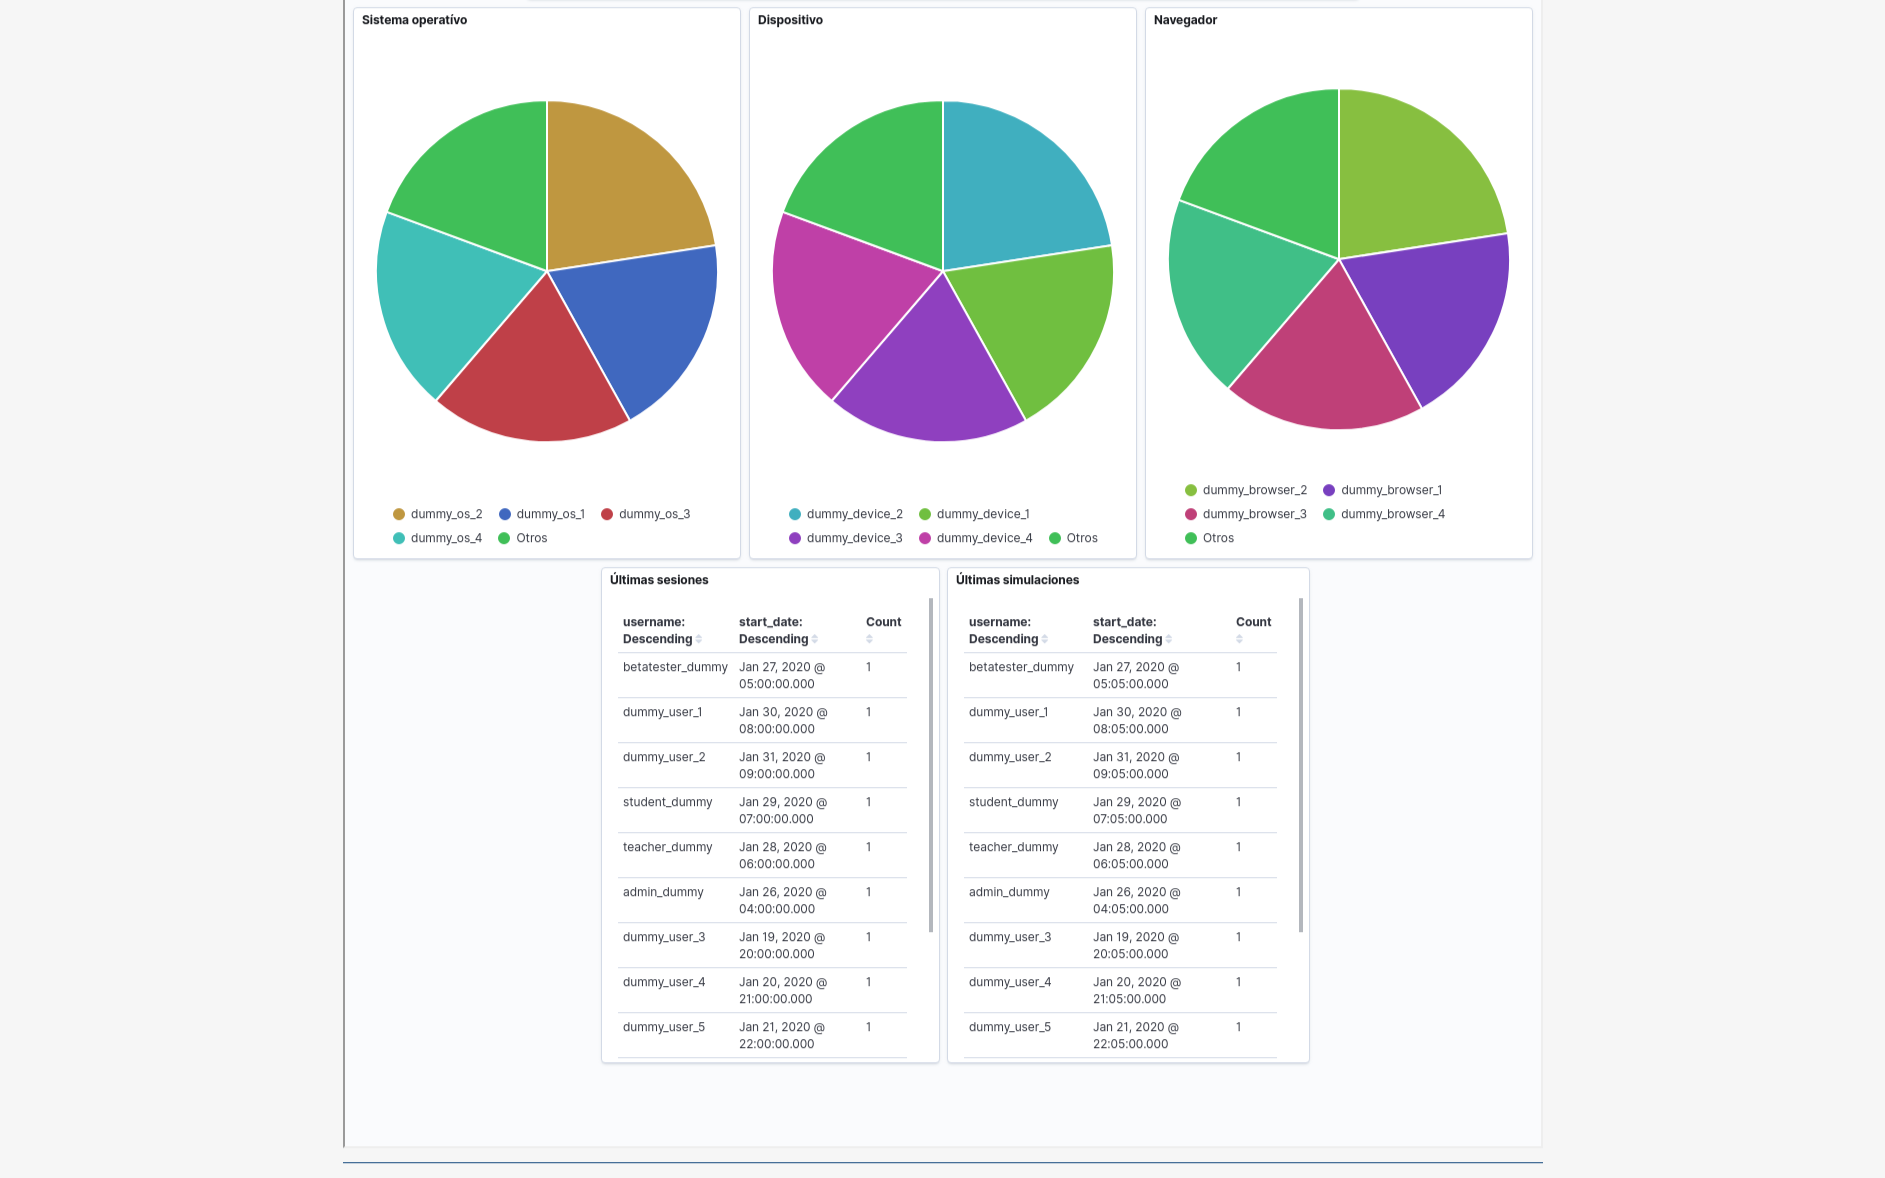
\includegraphics[width=10cm, keepaspectratio]{img/kibana_kibotics_03.png}
					\caption{Kibana en Kibotics parte 3}
					\label{fig:kibana_kibotics_03}
				\end{figure}
		\section{Despliegue en producción}
			(ELIMINAR?¿)
		\section{Generación de recursos de prueba para el desarrollo local}
			(INCOMPLETO? - ¿se puede evitar?)
			Para facilitar futuros desarrollos y ampliaciones de las mejoras de analíticas implementadas se han generado una serie de recursos para proveer al repositorio Github de herramientas.
			\subsection{Receta de instalación de Elasticsearch}
				Se ha incluido en el repositorio GitHub la receta necesaria para instalar la versión de Elasticsearch utilizada en producción.\\
				
				Con esto, se asegura que cualquier futuro desarrollador de la plataforma simplemente tenga que seguir la receta de instalación ahí explicitada para tener un entorno totalmente funcional.\\
				
			\subsection{Creación de bases de datos Dummy para Elasticsearch}
				Para proporcionar a los futuros desarrolladores datos realistas con los que poder empezar a trabajar sin necesidad de crearlos de manera manual, se ha creado una base de datos dummy la cual ofrece una variedad de datos para todos los índices utilizados tanto en este proyecto, como en otros desarrollos paralelos.\\
				
				Para la creación de esta base de datos de pruebas, se generó mediante un \textit{script} de Python el cual crea los índices y su estructura haciendo uso de la librería de que Elasticsearch proporciona para Python.\\
				
				El \textit{script} creará todos los índices con sus respectivas estructuras y tipologías de datos, un ejemplo, para el índice de sesiones es:
				
				\begin{Verbatim}[tabsize=4]
# Import librería Elasticsearch
from elasticsearch import Elasticsearch
client = Elasticsearch()

...

# JSON con la estructura del índice
session_mapping = {
	"settings": {
		"number_of_shards": 1,
		"number_of_replicas": 0
	},
	"mappings": {
		"properties": {
			"username": {
				"type":"keyword"
			},
			"start_date":{
				"type":"date"
			},
			"end_date":{
				"type":"date"
			},
			"duration": {
				"type":"double"
			},
			"client_ip":{
				"type":"ip"
			},
			"browser": {
				"type":"keyword"
			},
			"device":{
				"type":"keyword"
			},
			"location": {
				"type": "geo_point"
			},
			"os":{
				"type":"keyword"
			}
		}
	}
}

# Creación del índice en Elasticsearch
client.indices.create(
	index="kibotics_session_log",
	body=session_mapping,
	ignore=400
)
				\end{Verbatim}
				
				Una vez creadas las estructuras de los índices, el siguiente paso es guardar todos los objetos con la información de prueba que se deseé guardar.\\
				
				Finalizada la ejecución del \textit{script} ya tendríamos los datos en nuestro servicio local de Elasticsearch. Un problema que se encontró es que para ejecutar este \textit{script} es necesaria la instalación de varias librerías. Para simplificar aún más la instalación de la base de datos se han generado una serie de documentos \texttt{JSON} con la estructura y datos que otros usuarios importarán a su servicio Elasticsearch.\\
				
				Estos documentos JSON se han generado haciendo uso de la herramienta \texttt{elasticdump}, la cual tiene una instalación muy sencilla:
							
				\begin{Verbatim}[tabsize=4]
$ sudo npm install elasticdump -g
				\end{Verbatim}
				
				Para la generación de los documentos de datos y mapeo se han ejecutado las siguientes sentencias para cada uno de los índices usados en Elasticsearch:

				\begin{Verbatim}[tabsize=4]
$ elasticdump --input=http://127.0.0.1:9200/"INDEX_NAME" 
			--output="./mapping_elasticseach.json" --type=mapping
			
$ elasticdump --input=http://127.0.0.1:9200/"INDEX_NAME" 
			--output="./data_elasticsearch.json" --type=data

				\end{Verbatim}
				
				Para la importación de estos ficheros en la base de datos, el desarrollador simplemente tendrá que instalar \texttt{elasticdump} y ejecutar un \textit{script bash} el cual recorrerá y cargará todos los ficheros al servicio Elasticsearch local:
				
				\begin{Verbatim}[tabsize=4]
indexes="session simulation visit error classification ranking"
directory="./kibotics_dummy_es/"

for index in $indexes; do
	elasticdump --output=http://127.0.0.1:9200/"kibotics_"$index"_log" 
		--input=$directory"mapping_"$index"_es.json" --type=mapping

	elasticdump --output=http://127.0.0.1:9200/"kibotics_"$index"_log" 
		--input=$directory"data_"$index"_es.json" --type=data
done
				\end{Verbatim}
			\subsection{Receta de instalación de Kibana}
			Para completar la instalación de recursos del stack ELK utilizados en el proyecto se ha añadido la receta de instalación de Kibana.\\
						
			\subsection{Creación de bases de datos Dummy para Kibana}
			El proceso de exportación e importación de datos de prueba para Kibana es sencillo pues la propia interfaz gráfica de Kibana nos proporciona una herramienta para realizarlo.
			
			\begin{figure}[H]
				\centering
				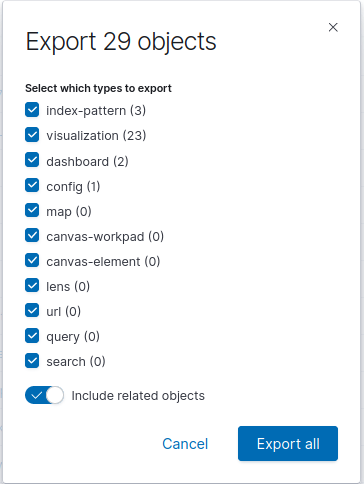
\includegraphics[width=7cm, keepaspectratio]{img/export_kibana.png}
				\caption{Exportación en interfaz Kibana.}
				\label{fig:export_kibana}
			\end{figure}
		
			Esta herramienta nos generará un fichero \texttt{NDJSON} similar a la estructura \texttt{JSON} con los patrones de índices creados, así como las visualizaciones, tablas o \textit{scripted fields} guardados en Kibana.\\
			
			Para que un futuro desarrollador importe estos datos simplemente podrá hacerlo por la interfaz gráfica de Kibana. Para unificar la metodología y ya que en el servidor de pre-producción/producción no se dispone de esta interfaz gráfica, esta también se puede realizar mediante la siguiente sentencia:\\
			

			
			\begin{Verbatim}[tabsize=4]
$ curl -X POST "localhost:5601/api/saved_objects/_import" -H "kbn-xsrf: true" 
	--form file=@kibotics_dummy_kibana.ndjson
			\end{Verbatim}
			
			


	\chapter{CONCLUSIONES}
		Finalmente, en este último capítulo se exponen las conclusiones alcanzadas, así como las competencias adquiridas durante la realización de este proyecto. Además, se plantean futuros trabajos de ampliación y mejora sobre el software desarrollado.
		\section{Conclusiones finales}
			Repasando lo definido en el capítulo 2, el principal objetivo de este proyecto es crear una herramienta en la que visualizar y analizar el estado de la aplicación Web Kibotics Webserver. Este objetivo se ha cumplido, se ha diseñado, desarrollado y testeado un módulo de analíticas en el que visualizar estos datos de uso de la aplicación.\\
			
			Adicionalmente a esto, se ha mejorado el sistema de registro de logs de la aplicación. Eliminando los ficheros de log indexados por días y creando una base de datos en ElastiSearch dividida en distintos índices sobre los que se registran variedad de eventos. Aumentando así la escalabilidad de este proceso de registro de logs y eventos, con lo que se consigue que esta sea una solución robusta y duradera.
		\section{Competencias adquiridas}
			En esta sección se enumeran las principales habilidades que se han adquirido en el desarrollo de este proyecto:
			\begin{itemize}
				\item Django y Python como herramientas muy potentes y accesibles para el desarrollo Web. Además, gracias a las librerías de las que estas disponen, son herramientas muy versátiles.\\
				
				\item Despliegue e implementación de diferentes tipos de bases de datos en un proyecto real. Importancia de la información para monitorizar un servicio Web.\\
				
				\item El stack ELK, ha sido una herramienta muy potente de la que he aprendido como es integrar varias tecnologías para crear un producto complejo, interconectado e interesante.\\
				
				\item GitHub, durante el desarrollo de este proyecto este repositorio ha estado siempre presente junto a la filosofía 'release often, release soon'.\\
				
				\item Trabajar en un software actualmente productivo sobre el que desarrollar para crear nuevas funcionalidades. Saber que no se dispone de los pasos a seguir y tener que investigar diferentes tecnologías para encontrar una solución óptima.\\
				 
				\item Una primera toma en contacto con el análisis de datos, sobre el que tendré que seguir aprendiendo y descubriendo nuevas tecnologías.\\
			\end{itemize}
			
		\section{Competencias empleadas}
			En el transcurso de este proyecto se han utilizado muchos de los conocimientos y habilidades adquiridos en el Grado, en especial en las asignaturas relacionadas con el desarrollo web. A continuación se enumerarán estas y otras asignaturas que me han aportado los conocimientos necesarios:
			
			\begin{itemize}
				\item Informática I, con el lenguaje ’Picky’ donde aprendí los fundamentos básicos de programación.	
				
				\item Informática II, en la que se llevaron a cabo proyectos más complejos, centrado en el aprendizaje de punteros y estructuras de datos complejas como tablas Hash. Haciendo uso del lenguaje ADA.	
						
				\item Protocolos de Transmisión de Audio y Vídeo en Internet, primera toma de contacto con Python y GithHub, herramientas imprescindibles para el desarrollo de este proyecto.
							
				\item Gráficos y visualización 3D, introducción al desarrollo web, centrado en JavaScript y el canvas HTML.			
			
				\item Construcción de Servicios y Aplicaciones Audiovisuales en Internet, asignatura muy importante en la que se profundizó en las 3 tecnologías web principales: JavaScript, HTML y CSS.
				
				\item Laboratorios en Tecnologías y Aplicaciones Web, ampliación de la anterior asignatura en la que aprendí a trabajar con frameworks web como NodeJS o Django, base de Kibotics Webserver.
			\end{itemize}
			
			
		\section{Trabajos futuros}
			En esta sección se proponen una serie de mejoras o ampliaciones con las que aumentar la funcionalidad del módulo de analíticas desarrollado:
			
			\begin{itemize}
				\item Kibotics Webserver es una aplicación grande y en constante ampliación, añadir mas sondas con las que tener la aplicación controlada será recomendable. Con estas nuevas sondas será necesaria la creación de nuevos índices y visualizaciones.\\
				
				\item Actualmente los datos almacenados en Elasticsearch solo pueden ser analizados accediendo al módulo desarrollado. Una herramienta automática que analice estos datos sería muy interesante para controlar, por ejemplo que todos los ejercicios están siendo accedidos y los tiempos de desarrollo de los usuarios no son demasiado elevados.\\
				
				\item El stack ELK posee, además de ElasticSeach y Kibana, otras herramientas muy interesantes como Logstash y Beats. Las cuales pueden dotar a ElasticSeach de nuevos datos procedentes de otras fuentes, como por ejemplo, logs del servidor con los que controlar los accesos que sufre la herramienta.\\
				
				\item Explorar otras mejoras de integración a la Web De Kibotics, ya que el Iframe no es algo ideal que tener en un servicio productivo por motivos de seguridad.\\
							
				\item El stack ELK es un software en constante evolución la cual añade nuevas y mejores funcionalidades constantemente. Mantener las versiones del software actualizadas es recomendable.\\
				
				\item Al proporcionar información muy sensible sobre el servicio, aumentar la seguridad en el servidor para acceder a estos datos es necesario.\\
			\end{itemize}
	
	
%		\chapter{REFERENCIAS}
%	
%
%	
%	HTML 
%	https://uniwebsidad.com/libros/xhtml/capitulo-1/breve-historia-de-html
%	https://www.w3schools.in/html-tutorial/history/
%	
%	SQLite
%	https://www.sqlite.org/about.html
%	
%	Elasticsearch
%	http://www.arquitectoit.com/elasticsearch/que-es-elasticsearch/
%	https://www.ionos.es/digitalguide/servidores/configuracion/que-es-elasticsearch/
%	https://www.elastic.co/guide/en/elastic-stack-get-started/7.6/get-started-elastic-stack.html\#install-elasticsearch
%		
%	
%	Kibana
%	https://www.elastic.co/es/what-is/kibana
%	
%
%	
%	\chapter{IMPLEMENTACIÓN DE MEJORAS PARA HERRAMIENTAS DE GESTIÓN}
%	\section{Asignación de permisos individuales}
	
	\begin{thebibliography}{7}
		
		
		\bibitem{HTML}
		\textit{Estandar HTML:}
		\url{https://html.spec.whatwg.org/}
	
		\bibitem{JavaScript}
		\textit{Documentación JavaScript MDN web docs:}
		\url{https://developer.mozilla.org/es/docs/Web/JavaScript}	
		
		\bibitem{Django MVC}
		\textit{Patrón Django Model-View-controller:}
		\url{https://uniwebsidad.com/libros/django-1-0/capitulo-5/el-patron-de-diseno-mtv}
		
		\bibitem{Django}
		\textit{Documentación \textit{Django Project}:}
		\url{https://www.djangoproject.com/}
		
		\bibitem{MongoDB}
		\textit{Documentación MongoDB:}
		\url{https://docs.mongodb.com/guides/server/introduction/}	
		
		\bibitem{Use_MongoDB}
		\textit{Quíen usa MongoDB:}
		\url{https://www.mongodb.com/who-uses-mongodb}
		
		\bibitem{elasticseach}
		\textit{Documentación Elasticseach:}
		\url{https://www.elastic.co/guide/en/elasticsearch/reference/current/index.html}
				
		\bibitem{versions_elasticsearch}
		\textit{Historico de versiones para Elasticsearch:}
		\url{https://www.elastic.co/downloads/past-releases#elasticsearch}	
		
				
		\bibitem{releases_matplotlib}
		\textit{Versiones de Matplotlib:}
		\url{https://github.com/matplotlib/matplotlib/releases}	
				
		\bibitem{kibana}
		\textit{Documentación Kibana:}
		\url{https://www.elastic.co/guide/en/kibana/current/index.html}	
				
		\bibitem{versions_kibana}
		\textit{Historico de versiones para Kibana:}
		\url{https://www.elastic.co/downloads/past-releases#kibana}	
				
		\bibitem{name}
		\textit{name:}
		\url{url}	
				
		\bibitem{name2}
		\textit{name2:}
		\url{url2}	
				
		\bibitem{name3}
		\textit{name3:}
		\url{url3}	
				
		\bibitem{name4}
		\textit{name4:}
		\url{url4}			
		

		\bibitem{Matplotlib}
		\textit{Documentación Matplotlib:}
		\url{https://matplotlib.org/}

		\bibitem{Elasticdump}
		\textit{Documentación Elasticdump:}
		\url{https://www.npmjs.com/package/elasticdump}	
	
	
	
	
		
	

	
	\end{thebibliography}

\end{document}